\documentclass[11pt,oneside]{article}

\usepackage[a4paper,margin=25mm,headheight=15pt]{geometry}
\usepackage[T1]{fontenc}
\usepackage[utf8]{inputenc}
\IfFileExists{libertinus.sty}{\usepackage{libertinus}}{\usepackage{lmodern}}
\usepackage{microtype}
\usepackage{amsmath,amssymb,amsthm,mathtools,mathrsfs,bm}
% Canonical mathematical notation for active FabiusFunction LaTeX documents.
%
% This file is intentionally a plain TeX input rather than a LaTeX package.
% Every standalone document loads it by an explicit path relative to that
% document's directory; included fragments inherit the definitions from their
% root document.  Keep this file independent of document layout and metadata.
%
% Contract:
%   * one command has one mathematical meaning throughout the active corpus;
%   * names encode semantic roles rather than a document-local choice of letter;
%   * visually similar but differently normalized objects have different print;
%   * every command below is defined normatively in the notation catalogue.
%
% The active corpus excludes docs/archive/.  Historical sources may retain
% their original notation only inside an explicitly labelled quotation.

\makeatletter
\@ifundefined{mathbb}{%
  \PackageError{fabius-notation}{The amssymb package must be loaded first}%
    {Load amsmath and amssymb before inputting fabius-notation.tex.}%
}{}
\@ifundefined{operatorname}{%
  \PackageError{fabius-notation}{The amsmath package must be loaded first}%
    {Load amsmath before inputting fabius-notation.tex.}%
}{}
\makeatother

% Version stamp used by the catalogue and by static audits.
\newcommand{\FabiusNotationVersion}{2026-08-31}

% Number systems.  NaturalNumbers is explicitly the nonnegative convention.
\newcommand{\NaturalNumbers}{\mathbb{N}_{0}}
\newcommand{\PositiveIntegers}{\mathbb{N}_{>0}}
\newcommand{\IntegerNumbers}{\mathbb{Z}}
\newcommand{\RationalNumbers}{\mathbb{Q}}
\newcommand{\RealNumbers}{\mathbb{R}}
\newcommand{\ComplexNumbers}{\mathbb{C}}
\newcommand{\ExtendedRealNumbers}{\overline{\mathbb{R}}}

% The three principal Fabius--Rvachev functions.  Subscripts are deliberate:
% a bare F and a calligraphic F have several unrelated uses in the corpus.
\newcommand{\FabiusBounded}{F_{\mathrm{bd}}}
\newcommand{\FabiusGlobal}{F_{\mathrm{gl}}}
\newcommand{\FabiusQuantile}{Q_{F}}
\newcommand{\FabiusClampedQuantile}{Q_{F,\mathrm{cl}}}
\newcommand{\RvachevUp}{\operatorname{up}}

% Constants, elementary operators, and delimiters.
\newcommand{\EulerE}{\mathrm{e}}
\newcommand{\ImaginaryUnit}{\mathrm{i}}
\newcommand{\Differential}{\mathop{}\!\mathrm{d}}
\newcommand{\AbsoluteValue}[1]{\left\lvert #1\right\rvert}
\newcommand{\Norm}[1]{\left\lVert #1\right\rVert}
\newcommand{\Floor}[1]{\left\lfloor #1\right\rfloor}
\newcommand{\Ceiling}[1]{\left\lceil #1\right\rceil}
\newcommand{\FractionalPart}[1]{\left\{#1\right\}}
\newcommand{\PositivePart}[1]{\left(#1\right)_{+}}
\newcommand{\IndicatorOf}[1]{\mathbf{1}_{#1}}
\newcommand{\SetOf}[1]{\left\{#1\right\}}
\newcommand{\InnerProduct}[1]{\left\langle #1\right\rangle}
\newcommand{\CardinalityOf}[1]{\left\lvert #1\right\rvert}
\newcommand{\DefinitionEquals}{\mathrel{\coloneqq}}
\newcommand{\Sign}{\operatorname{sgn}}
\newcommand{\IdentityOperator}{\operatorname{id}}
\newcommand{\SpanOperator}{\operatorname{span}}
\newcommand{\TraceOperator}{\operatorname{tr}}
\newcommand{\RankOperator}{\operatorname{rank}}
\newcommand{\DiagonalOperator}{\operatorname{diag}}
\newcommand{\ResidueOperator}{\operatorname*{Res}}
\newcommand{\LeastCommonMultiple}{\operatorname{lcm}}
\newcommand{\OrderOperator}{\operatorname{ord}}
\newcommand{\PrincipalLogarithm}{\operatorname{Log}}
\newcommand{\FallingFactorial}[2]{\left(#1\right)^{\underline{#2}}}
\newcommand{\RisingFactorial}[2]{\left(#1\right)^{\overline{#2}}}

% Support, topology, convolution, and metric notation.
\newcommand{\SupportOperator}{\operatorname{supp}}
\newcommand{\SupportOf}[1]{\SupportOperator\!\left(#1\right)}
\newcommand{\TopologicalSupportOf}[1]{\operatorname{tsupp}\!\left(#1\right)}
\newcommand{\Convolution}{\mathbin{*}}
\newcommand{\MetricDistance}{\operatorname{dist}}
\newcommand{\TotalVariationDistance}{d_{\mathrm{TV}}}

% Probability.  Equality and convergence in law are not metric distance.
\newcommand{\Probability}{\mathbb{P}}
\newcommand{\Expectation}{\mathbb{E}}
\newcommand{\Variance}{\operatorname{Var}}
\newcommand{\Covariance}{\operatorname{Cov}}
\newcommand{\LawOperator}{\operatorname{Law}}
\newcommand{\LawOf}[1]{\LawOperator\!\left(#1\right)}
\newcommand{\EqualInLaw}{\mathrel{\overset{\mathrm{law}}{=}}}
\newcommand{\ConvergesInLaw}{\mathrel{\xrightarrow{\mathrm{law}}}}

% Fourier and integral transforms.  The printed labels expose normalization.
% FourierTwoPi uses exp(-2*pi*i*x*xi); FourierAngular uses exp(-i*x*omega).
\newcommand{\FourierTwoPi}[1]{\widehat{#1}_{\,2\pi}}
\newcommand{\FourierAngular}[1]{\widehat{#1}_{\,\mathrm{ang}}}
\newcommand{\LaplaceTransformSymbol}{\mathcal{L}}
\newcommand{\MellinTransformSymbol}{\mathcal{M}}
\newcommand{\LaplaceTransformOf}[1]{\LaplaceTransformSymbol\!\left[#1\right]}
\newcommand{\MellinTransformOf}[1]{\MellinTransformSymbol\!\left[#1\right]}
\newcommand{\MomentGeneratingFunction}[1]{M_{#1}}
\newcommand{\CharacteristicFunction}[1]{\varphi_{#1}}

% The two standard sinc functions must never share one symbol.
\newcommand{\SincRad}{\operatorname{sinc}_{\mathrm{rad}}}
\newcommand{\SincPi}{\operatorname{sinc}_{\pi}}

% Binary arithmetic and Thue--Morse notation.
\newcommand{\BinaryDigitSum}{\operatorname{wt}_{2}}
\newcommand{\ThueMorseSignSymbol}{\varepsilon}
\newcommand{\ThueMorseSign}[1]{\varepsilon_{#1}}
\newcommand{\PadicValuation}[1]{\nu_{#1}}
\newcommand{\TwoAdicValuation}{\nu_{2}}

% q-series notation.  Every base is an explicit argument.
\newcommand{\QPochhammer}[3]{\left(#1;#2\right)_{#3}}
\newcommand{\GaussianBinomial}[3]{%
  \genfrac{[}{]}{0pt}{}{#1}{#2}_{#3}%
}
\newcommand{\QInteger}[2]{\left[#1\right]_{#2}}

% Named special functions.
\newcommand{\Polylogarithm}{\operatorname{Li}}
\newcommand{\LambertW}{W}
\newcommand{\GammaFunction}{\Gamma}
\newcommand{\RiemannZeta}{\zeta}

% Asymptotics.  BigO and LittleO are operator tokens for existing formula
% grammar; prefer the At forms so that the limiting regime is printed.
\newcommand{\BigO}{\mathcal{O}}
\newcommand{\LittleO}{o}
\newcommand{\BigOAt}[2]{\mathcal{O}_{#2}\!\left(#1\right)}
\newcommand{\LittleOAt}[2]{o_{#2}\!\left(#1\right)}

\usepackage{booktabs,longtable,tabularx,array,multirow}
\usepackage{graphicx}
\usepackage{caption}
\usepackage{float}
\usepackage{enumitem}
\usepackage{xcolor}
\usepackage{xurl}
\usepackage{hyperref}
\usepackage[nameinlink,capitalise,noabbrev]{cleveref}
\usepackage{fancyhdr}
\usepackage{listings}
\usepackage{siunitx}

\definecolor{navy}{HTML}{17365D}
\definecolor{teal}{HTML}{176B67}
\definecolor{burgundy}{HTML}{7A2848}
\definecolor{gold}{HTML}{9A6A0A}
\definecolor{slate}{HTML}{4B5968}
\definecolor{lightgray}{HTML}{F4F6F8}

\hypersetup{
  colorlinks=true,
  linkcolor=navy,
  citecolor=teal,
  urlcolor=burgundy,
  pdftitle={Matrix-Dilated Fabius--Rvachev Laws},
  pdfauthor={OpenAI GPT-5.6 Pro; report prepared for Vladimir Reshetnikov},
  pdfsubject={Infinite box splines, Thue--Morse derivative cubes, tensor cumulants, and rotating zonoid q-series},
  pdfkeywords={Fabius function, Rvachev up-function, Thue-Morse, box spline, zonoid, q-series, Bell polynomial, Bernoulli number, Legendre polynomial, Lambert W}
}

\pagestyle{fancy}
\fancyhf{}
\fancyhead[L]{\small\textsc{Matrix-dilated Fabius--Rvachev laws}}
\fancyhead[R]{\small\nouppercase{\leftmark}}
\fancyfoot[C]{\thepage}
\renewcommand{\headrulewidth}{0.4pt}

\setlength{\parindent}{0pt}
\setlength{\parskip}{0.50em}
\setlength{\emergencystretch}{3em}
\allowdisplaybreaks[3]
\setcounter{tocdepth}{2}
\setcounter{secnumdepth}{3}
\setlist[itemize]{leftmargin=1.9em,itemsep=0.25em,topsep=0.35em}
\setlist[enumerate]{leftmargin=2.2em,itemsep=0.25em,topsep=0.35em}
\graphicspath{{figures/}}
\captionsetup{font=small,labelfont=bf}

\newtheorem{theorem}{Theorem}[section]
\newtheorem{proposition}[theorem]{Proposition}
\newtheorem{lemma}[theorem]{Lemma}
\newtheorem{corollary}[theorem]{Corollary}
\newtheorem{conjecture}[theorem]{Conjecture}
\newtheorem{problem}[theorem]{Open problem}
\theoremstyle{definition}
\newtheorem{definition}[theorem]{Definition}
\newtheorem{example}[theorem]{Example}
\newtheorem{algorithm}[theorem]{Algorithm}
\theoremstyle{remark}
\newtheorem{remark}[theorem]{Remark}
\newtheorem{warning}[theorem]{Warning}

\newcommand{\vol}{\operatorname{vol}}
\newcommand{\Per}{\operatorname{Per}}
\newcommand{\Sym}{\operatorname{Sym}}
\newcommand{\diam}{\operatorname{diam}}
\newcommand{\AllOnesVector}{\boldsymbol{1}}
\newcommand{\AngularFourierStieltjesCoefficient}[2]{\operatorname{FSU}_{2\pi}\!\left[#1\right]\!\left[#2\right]}
\newcommand{\ip}[2]{\left\langle #1,#2\right\rangle}
\newcommand{\Repo}{\textcolor{navy}{\textbf{[repository input]}}}
\newcommand{\New}{\textcolor{teal}{\textbf{[proved here]}}}
\newcommand{\Derived}{\textcolor{gold}{\textbf{[derived synthesis]}}}
\newcommand{\Conj}{\textcolor{burgundy}{\textbf{[conjecture]}}}
\newcommand{\Num}{\textcolor{burgundy}{\textbf{[numerical]}}}

\newenvironment{statusbox}[1]{%
  \par\medskip\noindent\begin{center}\begin{minipage}{0.94\textwidth}
  \hrule\vspace{0.55em}\textbf{#1.}\quad
}{%
  \vspace{0.55em}\hrule\end{minipage}\end{center}\medskip
}

\lstdefinestyle{pythonstyle}{
  language=Python,
  basicstyle=\ttfamily\small,
  columns=fullflexible,
  keepspaces=true,
  showstringspaces=false,
  breaklines=true,
  frame=single,
  backgroundcolor=\color{lightgray},
  commentstyle=\itshape\color{slate},
  keywordstyle=\bfseries\color{navy},
  xleftmargin=0.4em,
  xrightmargin=0.4em
}

\title{\bfseries Matrix-Dilated Fabius--Rvachev Laws\\[0.35em]
\Large Infinite Box Splines, Thue--Morse Directional Derivatives,\\
Bell--Bernoulli Tensor Resolvents, and Rotating-Zonoid $q$-Series}
\author{Frontier research report prepared for Vladimir Reshetnikov\\
\small Repository-aware proofs and reproducible numerical experiments}
\date{30 August 2026\\
\small \texttt{ProveIt} snapshot \texttt{90b2d3587833dea1bc4a6bf0c36d92f7200396e6}}

\begin{document}
\maketitle

\begin{abstract}
The current \texttt{ProveIt} corpus develops the one-dimensional Fabius--Rvachev
system unusually far: exact dyadic arithmetic, Thue--Morse derivative trees,
$q$-binomial interpolation, infinite sinc products, Bell--Bernoulli moments,
Legendre and Appell representations, inverse-function jets, and phase-aware
Lambert--$W$ endpoint asymptotics are all already present.  This report moves in
a direction not found in the recursively audited LaTeX tree: an expansive matrix
replaces scalar dilation, and a finite vector dictionary replaces the single
uniform digit.

Let $A\in\mathrm{GL}_d(\RealNumbers)$ be expansive, let
$V=[v_1\ \cdots\ v_r]$, and let the vectors $U_n$ have independent
$\mathrm{Unif}[-1,1]$ coordinates.  We study
\[
 X_{A,V}=\sum_{n\ge1}A^{-n}VU_n.
\]
Its support is the self-affine infinite zonotope
$K_{A,V}=\sum_{n,j}[-A^{-n}v_j,A^{-n}v_j]$, while its Fourier transform is the
matrix-Mahler product
\[
 \Phi_{A,V}(\xi)=\prod_{n\ge1}\prod_{j=1}^r
 \SincRad\!\bigl(\ip{\xi}{A^{-n}v_j}\bigr),
 \qquad
 \Phi_{A,V}(A^T\xi)=\prod_j\SincRad\!\bigl(\ip{\xi}{v_j}\bigr)\Phi_{A,V}(\xi).
\]
A finite-orbit spanning condition is shown to be exactly the condition for a
full-dimensional compactly supported $C^\infty$ density.  The proof supplies a
log-Gaussian Fourier bound.  The limiting density is log-concave, while a simple
matrix-geometric criterion detects when it nevertheless has an exact central
plateau.  Finite prefixes are centered box splines and converge in every $C^m$
norm at a geometric rate; their first corrections are explicit Bell--Bernoulli
differential operators.

The scalar Thue--Morse derivative formula lifts to an exact multivariate cube.
After differentiating once along every generator in the first $N$ scales, the
density becomes a signed sum of $2^{rN}$ affine copies of itself, with signs
$(-1)^{\BinaryDigitSum(k)}$.  The same cube gives a tensor Prouhet identity annihilating every
polynomial of total degree below $rN$.  All joint cumulants are obtained from the
resolvent
\[
 \kappa_{2m}(X_{A,V})=
 \frac{2^{2m-1}B_{2m}}{m}
 (A^{\otimes 2m}-I)^{-1}\sum_{j=1}^r v_j^{\otimes 2m},
\]
and multivariate Bell partitions then give every moment.  This yields rationality
and denominator bounds for rational data, an exact Appell--Koopman intertwining
law, and explicit Legendre coefficients for every one-dimensional projection.

The planar family $A^{-1}=qR_\theta$ produces the most concrete new geometry.
Its support has perimeter $4\Norm v q/(1-q)$ and area
\[
 \frac{4\Norm v^2q^2}{1-q^2}
 \sum_{m\ge1}\AbsoluteValue{\sin(m\theta)}q^m.
\]
For rational $\theta/\pi$ this area series is rational in $q$; for irrational
$\theta/\pi$ the unit circle is its natural boundary.  Irrational supports have a
dense set of exposed edges whose union has full boundary length.  Nevertheless,
a natural Abel rescaling makes them converge to a Euclidean disk as $q\uparrow1$;
rational rotations instead converge to finite zonotopes.  Exact directional-cap
Laplace products connect this geometry back to inverse Fabius and Lambert--$W$
questions.  The irrational endpoint modulation is isolated as a conjectural
rotation-cocycle problem.  A fully commented Python program reproduces all
figures and numerical checks.
\end{abstract}

\tableofcontents
\newpage

\section{Corpus audit, contribution boundary, and notation}
\label{sec:audit}

\subsection{Recursive audit}

The report is pinned to commit
\texttt{90b2d3587833dea1bc4a6bf0c36d92f7200396e6} of
\url{https://github.com/VladimirReshetnikov/ProveIt}.  A recursive GitHub code
inventory returned 119 files with extension \texttt{.tex} under
\path{Analysis/FabiusFunction/docs}.  The tree contains current expositions,
large consolidated frontier volumes, same-day incoming reports, paper
transcriptions, and frozen historical copies.  Reading every frozen predecessor
as if it were an independent claim would overcount the corpus.  The audit
therefore used the repository's own \path{MANIFEST.md}, coverage tables, and
provenance notes to identify canonical descendants, and then searched the whole
recursive tree for exact and close variants of every proposed definition and
formula.

The most important current descendants inspected directly were the primary
Fabius--Rvachev exposition, the representation atlas, the exponent/$q$-series
volume, the inverse-and-sampling volume, the spectral-arithmetic volume, the
Thue--Morse atlas, the consolidated frontier reports, the mathematical glossary,
the Lean walkthrough, and the newest information-geometry report.  Targeted
whole-tree collision searches included
\begin{center}
\begin{tabular}{@{}ll@{}}
\toprule
Concept family & Search phrases and close variants \\
\midrule
matrix geometry & matrix dilation, self-affine, zonotope, zonoid, support function \\
multivariate splines & multivariate box spline, infinite box spline, matrix sinc product \\
tensor algebra & tensor cumulant, tensor Bell, Lyapunov cumulant, matrix Appell \\
rotating $q$-series & rotating support, $|\sin(n\theta)|$, natural boundary, Abel shape \\
directional endpoints & cap distribution, support deficit, rotation cocycle \\
\bottomrule
\end{tabular}
\end{center}
No occurrence of the defining matrix-dilated family, the rotating-zonoid area
series, its natural-boundary theorem, or the tensor Prouhet cube was found.  The
word ``new'' below consequently means \emph{new to this audited repository
snapshot}, not a claim of universal publication priority.

The external literature supplies important surrounding language.  Finite
prefixes belong to classical box-spline theory \cite{deBoorBoxSplines}; infinite
Minkowski sums of matrix-dilated segments occur as infinite zonotopes in
self-affine geometry \cite{ProtasovZaitseva}; and the finite zonotope volume
formula is classical \cite{GoverKrikorian}.  The contribution here is the
Fabius--Rvachev synthesis: smooth convolution laws on those supports, exact
matrix-Mahler and Rvachev equations, Thue--Morse derivative cubes,
Bell--Bernoulli tensor resolvents, rotating geometric $q$-series, and the
rational/irrational analytic dichotomies.

\begin{statusbox}{Status convention}
\Repo\ marks an imported fact already present in the repository or a classical
ingredient used with citation.  \New\ marks a statement proved in this report and
not located in the audited repository.  \Derived\ marks a useful consequence or
repackaging whose ingredients are standard.  \Conj\ marks an unproved statement.
Numerical evidence is always labeled \Num\ and is never used as a proof.
\end{statusbox}

\subsection{The scalar baseline}

The probabilistic normalization behind Rvachev's up-function is
\[
 X_2=\sum_{n\ge1}2^{-n}U_n,
 \qquad U_n\stackrel{\mathrm{iid}}\sim\mathrm{Unif}[-1,1].
\]
Its law has support $[-1,1]$, density $\RvachevUp$, and characteristic function
$\prod_{n\ge1}\SincRad(2^{-n}\xi)$, where throughout
\[
 \SincRad z=\begin{cases}\sin z/z,&z\ne0,\\1,&z=0.\end{cases}
\]
The bounded Fabius distribution on $[0,1]$ is obtained by the affine change of
variables $(X_2+1)/2$.  The repository already derives its dyadic arithmetic,
Thue--Morse formulas, exact moments, inverse asymptotics, and many transform
representations.  Our construction reduces to this law when $d=r=1$, $A=2$,
and $v_1=1$.

\subsection{Matrix notation}

Fix integers $d,r\ge1$.  Let $A\in\mathrm{GL}_d(\RealNumbers)$ be \emph{expansive}:
every eigenvalue of $A$ has modulus greater than one.  Put $B=A^{-1}$, let
$V=[v_1\ \cdots\ v_r]\in\RealNumbers^{d\times r}$, and let
$U_n=(U_{n,1},\ldots,U_{n,r})^T$ be independent vectors whose coordinates are
independent $\mathrm{Unif}[-1,1]$ variables.  Define
\begin{equation}
 X=X_{A,V}:=\sum_{n=1}^{\infty}B^nVU_n,
 \qquad g_{n,j}:=B^nv_j.
 \label{eq:defX}
\end{equation}
The law, characteristic function, moment generating function, and support will
be denoted by $\mu$, $\Phi$, $M$, and $K$ respectively.  For $g\in\RealNumbers^d$,
$D_g=\sum_a g_a\partial_a$ is the directional derivative.  Tensor powers are
symmetric whenever they occur as moments or cumulants; $\Sym$ denotes normalized
symmetrization.

\section{The matrix-dilated law and its self-affine support}
\label{sec:construction}

\begin{theorem}[Existence, exact support, and affine recursion]
\label{thm:existence-support}
\New\ The series \eqref{eq:defX} converges absolutely for every realization of
the bounded digits.  Its support is the compact centrally symmetric infinite
zonotope
\begin{equation}
 K=\sum_{n\ge1}\sum_{j=1}^r[-g_{n,j},g_{n,j}],
 \label{eq:support-zonotope}
\end{equation}
and its support function is
\begin{equation}
 h_K(w)=\sup_{x\in K}\ip{w}{x}
       =\sum_{n\ge1}\sum_{j=1}^r\AbsoluteValue{\ip{w}{g_{n,j}}}.
 \label{eq:support-function}
\end{equation}
If $X'$ is an independent copy of $X$ and $U$ is an independent uniform vector
on $[-1,1]^r$, then
\begin{equation}
 X\overset d=B(VU+X'),
 \qquad
 K=B\bigl(V[-1,1]^r+K\bigr).
 \label{eq:affine-recursion}
\end{equation}
Finally, $K$ has nonempty interior in $\RealNumbers^d$ exactly when
\begin{equation}
 \SpanOperator\{B^nv_j:n\ge1,\ 1\le j\le r\}=\RealNumbers^d.
 \label{eq:span-condition}
\end{equation}
\end{theorem}

\begin{proof}
Choose $\rho$ with $\rho(B)<\rho<1$.  There is $C_\rho$ such that
$\Norm{B^n}\le C_\rho\rho^n$.  Since
$\AbsoluteValue{U_{n,j}}\le1$,
\[
 \sum_{n,j}\Norm{B^nv_jU_{n,j}}
 \le C_\rho\sum_j\Norm{v_j}\sum_{n\ge1}\rho^n<\infty.
\]
The convergence is therefore deterministic and uniform on the compact product
space $\Omega=[-1,1]^{\NaturalNumbers\times r}$.

The summation map $S:\Omega\to\RealNumbers^d$ is continuous, and the product measure of
the digits has full support $\Omega$.  Hence the support of its pushforward is
the compact image $S(\Omega)$, which is exactly the Minkowski sum
\eqref{eq:support-zonotope}.  Support functions add under Minkowski addition and
the support function of $[-g,g]$ is $|\ip{w}{g}|$, proving
\eqref{eq:support-function}.  Splitting off the first scale gives
\[
 X=B\left(VU_1+\sum_{m\ge1}B^mVU_{m+1}\right),
\]
which proves the distributional and set recursions.

If the displayed span is proper, $K$ lies in that proper subspace.  Conversely,
if the span is all of $\RealNumbers^d$, some finite subcollection of generators is a basis;
their Minkowski sum contains a full-dimensional parallelotope, and therefore
$K$ has nonempty interior.
\end{proof}

\begin{remark}
The support theorem is stronger than the usual convex-hull statement for a
discrete self-affine attractor.  Uniform digits already fill each segment, so the
support itself, not merely its convex hull, is the infinite zonotope.  In the
one-generator case this support agrees with the infinite-zonotope convex hull
appearing in self-affine two-digit geometry \cite{ProtasovZaitseva}.
\end{remark}

\begin{corollary}[Exact projection support]
\label{cor:projection-support}
For every $w\in\RealNumbers^d$, the scalar projection $\ip{w}{X}$ has support
$[-h_K(w),h_K(w)]$.  In particular, widths and directional endpoint problems
are explicit before the density itself is known.
\end{corollary}

\begin{proof}
Project \eqref{eq:support-zonotope} under $x\mapsto\ip{w}{x}$.  The image
of a generator segment $[-g,g]$ is
\[
 [-|\ip{w}{g}|,|\ip{w}{g}|].
\]
Minkowski sums of centered intervals add their half-widths.
\end{proof}

\section{Fourier product, matrix Mahler equation, and smoothness}
\label{sec:fourier}

\begin{theorem}[Entire sinc product and matrix Mahler equation]
\label{thm:mahler}
\New\ The characteristic function extends to an entire function on $\ComplexNumbers^d$ and
has the locally uniformly convergent product
\begin{equation}
 \Phi(z)=\Expectation\EulerE^{\ImaginaryUnit\ip{z}{X}}
 =\prod_{n=1}^{\infty}\prod_{j=1}^r
   \SincRad\!\bigl(\ip{z}{B^nv_j}\bigr).
 \label{eq:fourier-product}
\end{equation}
It satisfies
\begin{equation}
 \Phi(A^Tz)=m_V(z)\Phi(z),
 \qquad
 m_V(z):=\prod_{j=1}^r\SincRad\!\bigl(\ip{z}{v_j}\bigr).
 \label{eq:matrix-mahler}
\end{equation}
Moreover,
\begin{equation}
 |\Phi(z)|\le \exp h_K(-\operatorname{Im}z),
 \label{eq:exp-type}
\end{equation}
so its exponential indicator is controlled exactly by the support zonoid.
\end{theorem}

\begin{proof}
Independence gives the finite products.  Since
$\SincRad u=1-u^2/6+O(u^4)$ locally and
$\sum_{n,j}\Norm{B^nv_j}^2<\infty$, the Weierstrass criterion gives local
uniform convergence on $\ComplexNumbers^d$ and hence an entire limit.  Substitution gives
\[
 \Phi(A^Tz)
 =\prod_{n,j}\SincRad\!\bigl(\ip{z}{AB^nv_j}\bigr)
 =\prod_j\SincRad\!\bigl(\ip{z}{v_j}\bigr)
  \prod_{n,j}\SincRad\!\bigl(\ip{z}{B^nv_j}\bigr).
\]
Finally, $|\EulerE^{\ImaginaryUnit\ip{z}{x}}|=\EulerE^{-\ip{\operatorname{Im}z}{x}}$ and
$x\in K$ almost surely, so expectation is bounded by the maximum over $K$,
which is \eqref{eq:exp-type}.
\end{proof}

\subsection{A finite-frame decay mechanism}

The one-dimensional up-product decays roughly like a Gaussian in $\log|\xi|$.
The same mechanism persists without a scalar order on the generators.  A finite
spanning block acts as a frame, and every matrix-dilated block contributes at
least one large sinc argument.

\begin{lemma}[Block-frame estimate]
\label{lem:block-frame}
Assume \eqref{eq:span-condition}.  Then there are an integer $L\ge1$ and $c>0$
such that
\begin{equation}
 \max_{1\le k\le L,\ 1\le j\le r}
 \AbsoluteValue{\ip{y}{B^kv_j}}\ge c\Norm y
 \qquad(y\in\RealNumbers^d).
 \label{eq:frame}
\end{equation}
For every $\beta>\rho(A)$ there is $C_\beta\ge1$ such that, for every block
index $m\ge0$ and every $\xi\in\RealNumbers^d$, one of the factors with
$n=mL+k$, $1\le k\le L$, has argument at least
\begin{equation}
 cC_\beta^{-1}\beta^{-mL}\Norm\xi.
 \label{eq:block-large}
\end{equation}
\end{lemma}

\begin{proof}
Choose $L$ so that the finite family in \eqref{eq:frame} spans $\RealNumbers^d$.
The maximum on the left, restricted to the unit sphere, is continuous and
strictly positive, giving $c$.  Since $\beta>\rho(A)$,
$\Norm{A^m}\le C_\beta\beta^m$.  Apply \eqref{eq:frame} to
$y=B^{TmL}\xi$.  Its norm is bounded below by
$\Norm\xi/\Norm{A^{TmL}}\ge C_\beta^{-1}\beta^{-mL}\Norm\xi$, and
\[
 \ip{B^{TmL}\xi}{B^kv_j}=\ip{\xi}{B^{mL+k}v_j}.
\]
\end{proof}

\begin{theorem}[Sharp dimensional dichotomy and log-Gaussian decay]
\label{thm:smoothness}
\New\ Let
$W=\SpanOperator\{B^nv_j:n\ge1,1\le j\le r\}$.  If $W\ne\RealNumbers^d$, then $\mu$ is
supported on a proper subspace and is singular with respect to $d$-dimensional
Lebesgue measure.  If $W=\RealNumbers^d$, then $\mu$ has a compactly supported
$C^\infty$ density $f$, and for every $\beta>\rho(A)$,
\begin{equation}
 |\Phi(\xi)|\le
 \exp\left
 \{-\frac{(\log\Norm\xi)^2}{2L\log\beta}+O(\log\Norm\xi)\right\}
 \qquad(\Norm\xi\to\infty),
 \label{eq:log-gaussian}
\end{equation}
where $L$ is any spanning-block length in \cref{lem:block-frame}.  In
particular, $\Norm\xi^N\Phi(\xi)$ is bounded for every $N$.
\end{theorem}

\begin{proof}
Only the full-span case remains.  On the real axis,
$|\SincRad t|\le\min(1,|t|^{-1})$.  Choose from each block the factor supplied by
\cref{lem:block-frame}.  Put $R=\Norm\xi$ and let $M$ be the largest integer for
which $cC_\beta^{-1}\beta^{-ML}R\ge1$.  Discarding all factors except one from
each block $0\le m\le M$ gives
\[
 |\Phi(\xi)|
 \le\prod_{m=0}^{M}\frac{C_\beta\beta^{mL}}{cR}.
\]
Taking logarithms,
\[
 \log|\Phi(\xi)|
 \le-(M+1)\log\frac{cR}{C_\beta}
     +\frac{L\log\beta}{2}M(M+1).
\]
Since $M=(\log R)/(L\log\beta)+O(1)$, this is
\eqref{eq:log-gaussian}.  The bound is faster than every negative power, so
$\xi\mapsto\xi^\alpha\Phi(\xi)$ is integrable for every multi-index $\alpha$.
Fourier inversion produces a $C^\infty$ density.  Its support is $K$ by
\cref{thm:existence-support}.
\end{proof}

\begin{remark}[Non-normal matrices]
No diagonalization, normality, or real spectrum is used.  The constant in
\eqref{eq:log-gaussian} records two genuinely matrix effects: the number $L$ of
scales needed to span, and a growth envelope $\beta$ for $A^m$.  Sharpening the
bound for non-normal $A$ should involve singular-value Lyapunov exponents rather
than the spectral-radius envelope; see \cref{prob:optimal-decay}.
\end{remark}

\subsection{Log-concavity survives the infinite matrix cascade}

\begin{theorem}[Log-concavity and convex superlevel sets]
\label{thm:logconcavity}
\New\ The probability measure $\mu$ is log-concave in the measure-theoretic
sense.  Under the span condition, its smooth density $f$ is log-concave on
$\RealNumbers^d$, is strictly positive on $\operatorname{int}K$, and vanishes off $K$.
Consequently every positive superlevel set $\{x:f(x)\ge c\}$ is compact and
convex.
\end{theorem}

\begin{proof}
Uniform probability on a segment is log-concave as a measure.  Affine images,
finite convolutions, and weak limits preserve log-concavity; these are standard
consequences of the Pr\'ekopa--Leindler theory \cite{Prekopa}.  Hence every
finite-prefix law $\mu_N$ is log-concave and, because $\mu_N\Rightarrow\mu$,
so is $\mu$.

When the generators span, \cref{thm:smoothness} gives a full-dimensional
continuous density.  The density characterization of a full-dimensional
log-concave measure supplies a log-concave representative.  It agrees almost
everywhere with $f$, hence everywhere on $\operatorname{int}K$ by continuity;
outside $K$ both vanish, and continuity forces the boundary value to be zero.
The positivity set of a full-dimensional log-concave density is the interior of
its convex support.  Convexity of positive superlevel sets is the defining
pointwise log-concavity inequality.
\end{proof}

\begin{remark}
Smoothness does not imply strict log-concavity.  A sufficiently dominant finite
prefix can leave a genuine flat core after convolution with the remaining tail.
The rotating family below makes this mechanism quantitative in
\cref{prop:plateau}.
\end{remark}

\section{The matrix Rvachev equation}
\label{sec:rvachev-equation}

Let $\sigma_g$ be the uniform probability measure on the segment $[-g,g]$.
As a distribution,
\begin{equation}
 D_g\sigma_g=\frac12(\delta_{-g}-\delta_g).
 \label{eq:segment-derivative}
\end{equation}
This elementary endpoint identity is the source of both Rvachev's differential
law and the Thue--Morse cube below.

\begin{theorem}[One-scale matrix Rvachev equation]
\label{thm:matrix-rvachev}
\New\ Assume the span condition, and let $f$ be the density from
\cref{thm:smoothness}.  Then
\begin{equation}
 \left(\prod_{j=1}^rD_{Bv_j}\right)f(x)
 =\frac{|\det A|}{2^r}
  \sum_{\omega\in\{0,1\}^r}(-1)^{|\omega|}
  f\bigl(Ax-V(2\omega-\AllOnesVector)\bigr).
 \label{eq:matrix-rvachev}
\end{equation}
For $d=r=1$, $A=2$, and $V=(1)$, it becomes
\begin{equation}
 \RvachevUp'(x)=2\bigl(\RvachevUp(2x+1)-\RvachevUp(2x-1)\bigr).
 \label{eq:scalar-rvachev}
\end{equation}
\end{theorem}

\begin{proof}
The one-step recursion factors the law as
\[
 \mu=\left(*_{j=1}^r\sigma_{Bv_j}\right)*(B_\#\mu).
\]
Apply one directional derivative to its matching segment factor and use
\eqref{eq:segment-derivative}.  Expanding the resulting $r$ endpoint choices
gives translations by
$BV(2\omega-\AllOnesVector)$ with signs $(-1)^{|\omega|}$.  The density of $B_\#\mu$ is
$|\det A|f(Ax)$, so translating and simplifying produces
\eqref{eq:matrix-rvachev}.  In the scalar case the left side is
$D_{1/2}\RvachevUp=\RvachevUp'/2$, and the displayed specialization follows.
\end{proof}

\begin{remark}
Equation \eqref{eq:matrix-rvachev} is a functional--differential equation on an
anisotropic expanding geometry.  The finite difference on the right is the
$r$-dimensional cube difference generated by the columns of $V$; the left is the
matching mixed directional derivative at the contracted scale.  It is therefore
a direct matrix analogue of the defining Rvachev mechanism, not merely a tensor
product of one-dimensional equations.
\end{remark}

\section{Finite box splines and all-orders geometric approximation}
\label{sec:box-splines}

Define
\begin{equation}
 X_N=\sum_{n=1}^NB^nVU_n,
 \qquad
 T_N=X-X_N,
 \qquad
 K_N=\sum_{n\le N,j}[-g_{n,j},g_{n,j}].
 \label{eq:prefix-tail}
\end{equation}
The law of $X_N$ is the centered box spline associated with the multiset of
$rN$ generators $g_{n,j}$; its Fourier transform is the corresponding finite
sinc product.  This is the standard probabilistic realization of a box spline
\cite{deBoorBoxSplines}.

\begin{proposition}[Exact head--tail self-similarity]
\label{prop:head-tail}
\New\ One has
\begin{equation}
 T_N\overset d=B^NX',
 \qquad
 \mu=\mu_N*(B^N_\#\mu),
 \qquad
 K=K_N+B^NK,
 \label{eq:head-tail}
\end{equation}
where $X'$ is an independent copy of $X$.  Consequently, for every $p\ge1$,
\begin{equation}
 W_p(\mu,\mu_N)
 \le \left(\Expectation\Norm{B^NX}^p\right)^{1/p}
 \le \sum_{n>N,j}\Norm{g_{n,j}},
 \label{eq:wasserstein}
\end{equation}
and the same last quantity bounds the Hausdorff distance $d_H(K,K_N)$.
\end{proposition}

\begin{proof}
Reindex the tail and use the same digit law.  The coupling $(X,X_N)$ gives the
Wasserstein estimate, while the deterministic tail norm gives the final bound.
The support identity follows from Minkowski addition.
\end{proof}

For the differential expansion define the tail power tensors
\begin{equation}
 Q_{k,N}:=\sum_{n>N}\sum_{j=1}^r g_{n,j}^{\otimes k},
 \qquad
 S_{k,N}:=\sum_{n>N,j}\Norm{g_{n,j}}^k.
 \label{eq:tail-tensors}
\end{equation}
Thus $Q_{2,N}$ is three times the tail covariance.  If
$\rho(B)<\rho<1$, then $S_{k,N}=O(\rho^{kN})$.

\begin{theorem}[$C^m$ convergence and the first two correction layers]
\label{thm:Cm-expansion}
\New\ Assume the span condition.  For every fixed $m\ge0$, the finite box-spline
density $f_N$ is $C^{m+6}$ once $N$ is sufficiently large, and
\begin{align}
 f={}&f_N+\frac16\,Q_{2,N}:D^2f_N+O_{C^m}(S_{2,N}^2),
 \label{eq:first-correction}\\
 f={}&f_N+\frac16\,Q_{2,N}:D^2f_N
 -\frac1{180}\sum_{n>N,j}D_{g_{n,j}}^4f_N
 +\frac1{72}(Q_{2,N}:D^2)^2f_N
 +O_{C^m}(S_{2,N}^3).
 \label{eq:second-correction}
\end{align}
Here $Q:D^2=\sum_{a,b}Q_{ab}\partial_a\partial_b$.  In particular,
$\Norm{f-f_N}_{C^m}=O(\rho^{2N})$ for every $\rho>\rho(B)$.
\end{theorem}

\begin{proof}
Choose a fixed prefix $N_0$ containing sufficiently many spanning blocks that
$|\Phi_{N_0}(\xi)|\le C(1+\Norm\xi)^{-m-2k-d-2}$ for the needed value of $k$.
The block argument of \cref{thm:smoothness}, stopped after finitely many blocks,
gives such a prefix.  For $N\ge N_0$, every additional real sinc factor has
modulus at most one, so $\Phi_N$ inherits this integrable majorant.

The tail multiplier is
\[
 \Psi_N(\xi)=\prod_{n>N,j}\SincRad\ip{\xi}{g_{n,j}}.
\]
The cumulant expansion of a uniform digit begins
\[
 \log\SincRad t=-\frac{t^2}{6}-\frac{t^4}{180}+O(t^6).
\]
Therefore
\[
 \Psi_N(\xi)=1-\frac16Q_{2,N}[\xi,\xi]
 -\frac1{180}\sum_{n>N,j}\ip{\xi}{g_{n,j}}^4
 +\frac1{72}Q_{2,N}[\xi,\xi]^2
 +O(\Norm\xi^6S_{2,N}^3).
\]
The same estimate can be made global by increasing the constant, because
$|1-\SincRad t|\le Ct^2$ and the sixth-order Taylor remainder is bounded by
$C|t|^6$.  Multiply by $\Phi_N$, integrate against $\Norm\xi^m$, and use the
fixed integrable majorant.  Under the convention
$\FourierAngular{f}(-\xi)=\int\EulerE^{\ImaginaryUnit\ip{\xi}{x}}f(x)\Differential x$, multiplication by
$-\ip{\xi}{g}^2$ is the Fourier image of $D_g^2$, giving
\eqref{eq:first-correction} and \eqref{eq:second-correction}.
\end{proof}

\subsection{The Bell--Bernoulli operator to arbitrary order}

Let
\begin{equation}
 c_{2m}:=\kappa_{2m}(U)
 =\frac{2^{2m-1}B_{2m}}{m},
 \qquad c_{2m+1}=0,
 \label{eq:uniform-cumulants}
\end{equation}
for $U\sim\mathrm{Unif}[-1,1]$.  The tail multiplier has the exact local
logarithm
\begin{equation}
 \log\Psi_N(\xi)
 =\sum_{m\ge1}\frac{c_{2m}}{(2m)!}
   (\ImaginaryUnit)^{2m}\sum_{n>N,j}\ip{\xi}{g_{n,j}}^{2m}.
 \label{eq:tail-log}
\end{equation}
Thus the formal differential operator
\begin{equation}
 \mathcal L_N
 =\sum_{m\ge1}\frac{c_{2m}}{(2m)!}
  \sum_{n>N,j}D_{g_{n,j}}^{2m}
 \label{eq:tail-operator}
\end{equation}
obeys $f\sim\exp(\mathcal L_N)f_N$.  Expanding the exponential uses complete
Bell polynomials.  The proof of \cref{thm:Cm-expansion} extends verbatim: after
retaining all terms of geometric degree at most $2M$, the $C^m$ remainder is
$O(\rho^{(2M+2)N})$.  This is a matrix-valued counterpart of the Bell--Bernoulli
finite-sinc expansions already developed in the scalar repository.

\section{The multivariate Thue--Morse derivative cube}
\label{sec:thue-morse}

Order the first $N$ scales' generators as
$g_1,\ldots,g_M$, where $M=rN$.  For
$\omega=(\omega_1,\ldots,\omega_M)\in\{0,1\}^M$, put
\begin{equation}
 s_\omega=\sum_{\ell=1}^M(2\omega_\ell-1)g_\ell,
 \qquad \varepsilon_\omega=(-1)^{|\omega|}.
 \label{eq:cube-points}
\end{equation}
When the bit strings are ordered by their binary integers, $\varepsilon_\omega$
is the Prouhet--Thue--Morse sign.

\begin{theorem}[Exact derivative cube]
\label{thm:derivative-cube}
\New\ In the sense of distributions,
\begin{equation}
 \left(\prod_{\ell=1}^M D_{g_\ell}\right)\mu
 =2^{-M}\sum_{\omega\in\{0,1\}^M}
   \varepsilon_\omega\,\tau_{s_\omega}(B^N_\#\mu),
 \label{eq:measure-cube}
\end{equation}
where $\tau_s\nu$ denotes translation by $s$.  Under the span condition this is
the pointwise smooth identity
\begin{equation}
 \left(\prod_{\ell=1}^M D_{g_\ell}\right)f(x)
 =\frac{|\det A|^N}{2^M}
  \sum_{\omega\in\{0,1\}^M}\varepsilon_\omega
  f\bigl(A^N(x-s_\omega)\bigr).
 \label{eq:density-cube}
\end{equation}
\end{theorem}

\begin{proof}
Factor $\mu$ into the $M$ segment measures and the tail $B^N_\#\mu$.  Assign
$D_{g_\ell}$ to the matching segment measure and use
\eqref{eq:segment-derivative}.  Expanding the endpoint choices gives
\eqref{eq:measure-cube}.  The tail density is
$|\det A|^Nf(A^Nx)$, yielding \eqref{eq:density-cube}.
\end{proof}

\begin{corollary}[Tensor Prouhet cancellation]
\label{cor:tensor-prouhet}
\New\ The cube points satisfy the exponential identity
\begin{equation}
 \sum_{\omega}\varepsilon_\omega\EulerE^{\ip{z}{s_\omega}}
 =(-2)^M\prod_{\ell=1}^M\sinh\ip{z}{g_\ell}.
 \label{eq:exponential-prouhet}
\end{equation}
Consequently,
\begin{equation}
 \sum_\omega\varepsilon_\omega s_\omega^{\otimes k}=0
 \quad(0\le k<M),
 \label{eq:tensor-vanishing}
\end{equation}
and at the first surviving degree
\begin{equation}
 \sum_\omega\varepsilon_\omega s_\omega^{\otimes M}
 =(-2)^MM!\,\Sym(g_1\otimes\cdots\otimes g_M).
 \label{eq:first-tensor}
\end{equation}
Equivalently, the signed cube annihilates every polynomial on $\RealNumbers^d$ of total
degree less than $M$.
\end{corollary}

\begin{proof}
The left side factors coordinate by coordinate as
\[
 \prod_{\ell=1}^M
 \left(\EulerE^{-\ip{z}{g_\ell}}-\EulerE^{\ip{z}{g_\ell}}\right),
\]
which is \eqref{eq:exponential-prouhet}.  Compare homogeneous Taylor terms at
$z=0$.  The product of $M$ hyperbolic sines has no term below degree $M$, and
its degree-$M$ term is $\prod_\ell\ip{z}{g_\ell}$.  Polarization gives
\eqref{eq:first-tensor}.
\end{proof}

\begin{remark}[Why this is genuinely multivariate]
The signs are still the one-dimensional Thue--Morse character of the Boolean
cube, but the nodes are not a scalar dyadic grid.  They are vertices of an
anisotropic matrix-generated zonotope, and the first nonzero tensor records the
entire ordered generator geometry.  Tensor-product Fabius laws appear only when
$A$ and $V$ split into invariant coordinate blocks.
\end{remark}

\section{Bell--Bernoulli tensor cumulants and arithmetic}
\label{sec:cumulants}

For $t$ near zero, the cumulant generating function is
\begin{equation}
 \log M(t)
 =\sum_{n,j}\log\frac{\sinh\ip{t}{g_{n,j}}}{\ip{t}{g_{n,j}}}.
 \label{eq:cgf}
\end{equation}
The scalar Bernoulli expansion in \eqref{eq:uniform-cumulants} can be summed
exactly over matrix scales.

\begin{theorem}[Tensor resolvent formula]
\label{thm:tensor-resolvent}
\New\ Every odd cumulant tensor of $X$ vanishes.  For $m\ge1$,
\begin{equation}
 \boxed{\quad
 \kappa_{2m}(X)
 =c_{2m}(A^{\otimes 2m}-I)^{-1}
   \sum_{j=1}^r v_j^{\otimes 2m}.
 \quad}
 \label{eq:tensor-resolvent}
\end{equation}
Equivalently, it is the unique symmetric tensor solving the higher Lyapunov
equation
\begin{equation}
 (A^{\otimes 2m}-I)\kappa_{2m}(X)
 =c_{2m}\sum_jv_j^{\otimes 2m}.
 \label{eq:higher-lyapunov}
\end{equation}
In particular, the covariance matrix $\Sigma$ is the unique solution of
\begin{equation}
 A\Sigma A^T-\Sigma=\frac13VV^T.
 \label{eq:lyapunov}
\end{equation}
\end{theorem}

\begin{proof}
Cumulants add over independent summands and transform tensorially under linear
maps.  Hence
\[
 \kappa_k(X)=c_k\sum_{n\ge1}\sum_j(B^nv_j)^{\otimes k}
 =c_k\sum_{n\ge1}(B^{\otimes k})^n\sum_jv_j^{\otimes k}.
\]
All eigenvalues of $B^{\otimes k}$ have modulus below one, so the geometric
operator series equals
\[
 (I-B^{\otimes k})^{-1}B^{\otimes k}
 =(A^{\otimes k}-I)^{-1}.
\]
This proves \eqref{eq:tensor-resolvent}.  For $k=2$, interpret the tensor equation
as a matrix identity and use $c_2=1/3$.
\end{proof}

\begin{corollary}[All joint moments by set partitions]
\label{cor:bell-moments}
\New\ Let $\Pi_k$ be the set of set partitions of $\{1,\ldots,k\}$.  Then
\begin{equation}
 \Expectation X^{\otimes k}
 =\sum_{\pi\in\Pi_k}\Sym
   \bigotimes_{C\in\pi}\kappa_{|C|}(X).
 \label{eq:set-partition-moments}
\end{equation}
For a projection $Y_w=\ip{w}{X}$, put
$\lambda_k(w)=\ip{\kappa_k(X)}{w^{\otimes k}}$.  Its scalar moments are the
complete Bell polynomials
\begin{equation}
 \Expectation Y_w^k=\mathcal B_k(\lambda_1(w),\ldots,\lambda_k(w)).
 \label{eq:bell-projection}
\end{equation}
\end{corollary}

\begin{proof}
This is the classical moment--cumulant relation, written in symmetric tensor
notation; see McCullagh's tensor treatment \cite{McCullagh}.  Contracting with
$w^{\otimes k}$ gives the scalar complete Bell polynomial.
\end{proof}

\begin{corollary}[Rational and algebraic arithmetic]
\label{cor:arithmetic}
\New\ If $A$ and $V$ have entries in a number field $K_0$, then every joint
moment of $X$ lies in $K_0$.  In particular, rational data give rational moments.
If $A$ and $V$ are integral, every coordinate of
\begin{equation}
 \frac{\det(A^{\otimes 2m}-I)}{c_{2m}}\,\kappa_{2m}(X)
 \label{eq:integer-adjugate}
\end{equation}
is an integer.  Thus the denominator of each order-$2m$ cumulant divides the
Bernoulli denominator of $c_{2m}$ times
$|\det(A^{\otimes 2m}-I)|$; Bell partitions give an explicit, though generally
non-sharp, denominator bound for every moment.
\end{corollary}

\begin{proof}
The matrix in \eqref{eq:tensor-resolvent} is invertible because every eigenvalue
of $A^{\otimes k}$ has modulus greater than one.  Field closure under inversion
proves the first assertion.  For integral data, use the adjugate formula for the
inverse of $A^{\otimes 2m}-I$ and then \eqref{eq:set-partition-moments}.
\end{proof}

\begin{remark}
The scalar dyadic moment denominators in the repository possess far subtler
$2$-adic structure than this generic determinant bound.  The matrix formula
identifies the new arithmetic object that should replace the factors
$2^{2m}-1$: the determinant and invariant factors of $A^{\otimes 2m}-I$.
Smith normal form, rather than a single valuation, is the natural next layer.
\end{remark}

\section{Appell--Koopman structure and Legendre projections}
\label{sec:appell-legendre}

\subsection{A matrix Appell intertwiner}

Define the averaging operator on polynomials by
\begin{equation}
 (Tp)(x)=\Expectation\,p\bigl(B(x+VU)\bigr),
 \label{eq:transfer-operator}
\end{equation}
where $U$ is uniform on $[-1,1]^r$.  Define the multivariate Appell generating
function
\begin{equation}
 \mathcal A(x,t)=\frac{\EulerE^{\ip{t}{x}}}{M(t)}
 =\sum_{k\ge0}\frac1{k!}
  \ip{\mathbf A_k(x)}{t^{\otimes k}}.
 \label{eq:appell-generating}
\end{equation}
The tensors $\mathbf A_k$ are polynomial-valued and begin with
$\mathbf A_0=1$, $\mathbf A_1=x$, and
$\mathbf A_2=x^{\otimes2}-\Sigma$.

\begin{theorem}[Exact Appell--Koopman intertwining]
\label{thm:appell}
\New\ The generating function obeys
\begin{equation}
 T\mathcal A(x,t)=\mathcal A(x,B^Tt),
 \label{eq:appell-intertwine}
\end{equation}
and therefore
\begin{equation}
 T\mathbf A_k=(B^{\otimes k})\mathbf A_k.
 \label{eq:appell-tensor-action}
\end{equation}
If $A$ is diagonalizable over $\ComplexNumbers$, contraction of $\mathbf A_k$ with symmetric
tensor products of left eigenvectors gives a complete Appell eigenbasis for
polynomials.  The degree-$k$ eigenvalues are products of $k$ eigenvalues of
$B=A^{-1}$.
\end{theorem}

\begin{proof}
The affine fixed-point equation implies
\begin{equation}
 M(t)=M(B^Tt)\prod_{j=1}^r
 \frac{\sinh\ip{B^Tt}{v_j}}{\ip{B^Tt}{v_j}}.
 \label{eq:mgf-mahler}
\end{equation}
Using this identity in \eqref{eq:transfer-operator},
\[
 T\mathcal A(x,t)
 =\frac{\EulerE^{\ip{B^Tt}{x}}}{M(t)}
  \prod_j\frac{\sinh\ip{B^Tt}{v_j}}{\ip{B^Tt}{v_j}}
 =\frac{\EulerE^{\ip{B^Tt}{x}}}{M(B^Tt)}.
\]
Compare homogeneous coefficients in $t$.  Since Appell tensors are monic by
\eqref{eq:appell-generating}, they form a triangular basis of the polynomial
algebra; diagonalizing $B$ gives the final assertion.  For background on Appell
families and their multivariate relatives, see \cite{Anshelevich}.
\end{proof}

\subsection{Exact Legendre coefficients of every projection}

Fix $w\ne0$, put $h=h_K(w)$, and normalize
$Y=\ip{w}{X}/h\in[-1,1]$.  Under the span condition, $Y$ has a smooth compactly
supported density $p_w$ on $[-1,1]$.  Write
\begin{equation}
 p_w(y)=\sum_{\ell=0}^{\infty}a_\ell(w)P_\ell(y)
 \label{eq:legendre-expansion}
\end{equation}
in $L^2[-1,1]$ and, in fact, with rapid coefficient decay.

\begin{proposition}[Bell--Bernoulli--Legendre bridge]
\label{prop:legendre}
\New\ The exact coefficient is
\begin{equation}
 a_\ell(w)=\frac{2\ell+1}{2}\Expectation P_\ell(Y).
 \label{eq:legendre-coefficient}
\end{equation}
Using
\begin{equation}
 P_\ell(y)=2^{-\ell}\sum_{k=0}^{\Floor{\ell/2}}
 (-1)^k\frac{(2\ell-2k)!}{k!(\ell-k)!(\ell-2k)!}
 y^{\ell-2k},
 \label{eq:legendre-monomial}
\end{equation}
all coefficients are finite expressions in the tensor resolvents
\eqref{eq:tensor-resolvent} and complete Bell polynomials
\eqref{eq:bell-projection}.  Every odd coefficient vanishes.  The first even
ones are
\begin{align}
 a_0&=\frac12,\nonumber\\
 a_2&=\frac54\left(3\Expectation Y^2-1\right),\nonumber\\
 a_4&=\frac9{16}\left(35\Expectation Y^4-30\Expectation Y^2+3\right).
 \label{eq:first-legendre}
\end{align}
\end{proposition}

\begin{proof}
Orthogonality gives \eqref{eq:legendre-coefficient}; insert
\eqref{eq:legendre-monomial} and use \cref{cor:bell-moments}.  The law is
centrally symmetric, so odd moments and odd Legendre coefficients vanish.
\end{proof}

\begin{remark}
This bridge does not assert that the multivariate density itself has a preferred
basis of products of Legendre polynomials.  It says something more invariant:
every Radon projection has an exact scalar Legendre expansion whose coefficients
are contractions of matrix resolvents.  The direction $w$ enters through both
the support gauge $h_K(w)$ and the tensor contractions.
\end{remark}

\section{Zonoid volume and the geometry carried by the density}
\label{sec:zonoid}

\begin{theorem}[Infinite-zonotope volume formula]
\label{thm:volume}
\New\ Enumerate all generators in \eqref{eq:support-zonotope} as
$(g_\ell)_{\ell\ge1}$.  Then
\begin{equation}
 \vol_d(K)=2^d\sum_{1\le\ell_1<\cdots<\ell_d}
 \AbsoluteValue{\det(g_{\ell_1},\ldots,g_{\ell_d})}.
 \label{eq:infinite-volume}
\end{equation}
The series converges absolutely.  It is positive exactly under the span
condition.
\end{theorem}

\begin{proof}
For the finite zonotope generated by $g_1,\ldots,g_M$, the classical zonotope
formula is
\[
 2^d\sum_{\ell_1<\cdots<\ell_d}
 |\det(g_{\ell_1},\ldots,g_{\ell_d})|;
\]
see \cite{GoverKrikorian}.  Absolute convergence follows from
$|\det(g_{\ell_1},\ldots,g_{\ell_d})|\le\prod_i\Norm{g_{\ell_i}}$ and
$\sum_\ell\Norm{g_\ell}<\infty$.  The finite zonotopes converge to $K$ in
Hausdorff distance, and volume is continuous under Hausdorff convergence of
convex compact sets.  Positivity is equivalent to the existence of a nonzero
$d\times d$ minor, hence to spanning.
\end{proof}

\begin{corollary}[A determinant series for matrix-dilated support volume]
\label{cor:matrix-volume}
For \eqref{eq:defX},
\begin{equation}
 \vol_d(K)=2^d\sum_{
 (n_1,j_1)<\cdots<(n_d,j_d)}
 \AbsoluteValue{\det(B^{n_1}v_{j_1},\ldots,B^{n_d}v_{j_d})}.
 \label{eq:matrix-volume}
\end{equation}
Thus support volume is a convergent matrix $q$-series in the singular geometry
of powers of $B$.
\end{corollary}

\section{The rotating planar family}
\label{sec:rotating}

Set $d=2$, $r=1$, choose $0<q<1$, an angle $\theta$, and a nonzero vector $v$.
Let $R_\theta$ denote counterclockwise rotation and define
\begin{equation}
 X_{q,\theta}=\sum_{n\ge1}q^nR_{n\theta}v\,U_n.
 \label{eq:rotating-law}
\end{equation}
This is the matrix law with
$B=qR_\theta$ and $A=q^{-1}R_{-\theta}$.  It is collinear only when
$\theta\in\pi\IntegerNumbers$; otherwise it has a $C^\infty$ density.

\begin{proposition}[Rotating Mahler and Rvachev equations]
\label{prop:rotating-equations}
\New\ The characteristic function and density satisfy
\begin{align}
 \Phi(q^{-1}R_\theta\xi)
 &=\SincRad\ip{\xi}{v}\,\Phi(\xi),
 \label{eq:rotating-mahler}\\
 D_{qR_\theta v}f(x)
 &=\frac1{2q^2}
 \left[f(q^{-1}R_{-\theta}x+v)
       -f(q^{-1}R_{-\theta}x-v)\right].
 \label{eq:rotating-rvachev}
\end{align}
\end{proposition}

\begin{proof}
Specialize \cref{thm:mahler,thm:matrix-rvachev}, noting that
$|\det A|=q^{-2}$.
\end{proof}

\subsection{Perimeter and area as exact \texorpdfstring{$q$}{q}-series}

Write $a=\Norm v$.  The support is
\begin{equation}
 K_{q,\theta}=\sum_{n\ge1}[-q^nR_{n\theta}v,q^nR_{n\theta}v].
 \label{eq:rotating-support}
\end{equation}

\begin{theorem}[Exact support function, perimeter, and area]
\label{thm:rotating-geometry}
\New\ If $w_\varphi=(\cos\varphi,\sin\varphi)$ and $v$ has angle $\varphi_0$,
then
\begin{equation}
 h_{q,\theta}(\varphi)
 =a\sum_{n\ge1}q^n
   \AbsoluteValue{\cos(n\theta+\varphi_0-\varphi)}.
 \label{eq:rotating-support-function}
\end{equation}
The perimeter is independent of $\theta$:
\begin{equation}
 \Per(K_{q,\theta})=\frac{4aq}{1-q}.
 \label{eq:rotating-perimeter}
\end{equation}
The area is
\begin{equation}
 \boxed{\quad
 \operatorname{Area}(K_{q,\theta})
 =\frac{4a^2q^2}{1-q^2}
  \sum_{m=1}^{\infty}\AbsoluteValue{\sin(m\theta)}q^m.
 \quad}
 \label{eq:rotating-area}
\end{equation}
The $N$-stage formulas are
\begin{align}
 \Per(K_N)&=\frac{4aq(1-q^N)}{1-q},
 \label{eq:finite-perimeter}\\
 \operatorname{Area}(K_N)
 &=\frac{4a^2q^2}{1-q^2}
 \sum_{m=1}^{N-1}q^m\AbsoluteValue{\sin(m\theta)}
       \left(1-q^{2(N-m)}\right).
 \label{eq:finite-area}
\end{align}
\end{theorem}

\begin{proof}
The support function is \eqref{eq:support-function}.  In the plane, the
perimeter of a Minkowski sum is the sum of perimeters, and the degenerate segment
$[-g,g]$ contributes $4\Norm g$; approximation by thin rectangles justifies this
convention directly.  Summing $4aq^n$ gives \eqref{eq:rotating-perimeter}.

The two-dimensional case of \eqref{eq:infinite-volume} gives
\[
 \operatorname{Area}(K)
 =4\sum_{1\le n<k}q^{n+k}a^2\AbsoluteValue{\sin((k-n)\theta)}.
\]
Group by $m=k-n$ and sum $\sum_{n\ge1}q^{2n}=q^2/(1-q^2)$ to obtain
\eqref{eq:rotating-area}.  Stopping at $k\le N$ gives
$\sum_{n=1}^{N-m}q^{2n}=q^2(1-q^{2(N-m)})/(1-q^2)$ and hence
\eqref{eq:finite-area}.
\end{proof}

\begin{figure}[H]
\centering
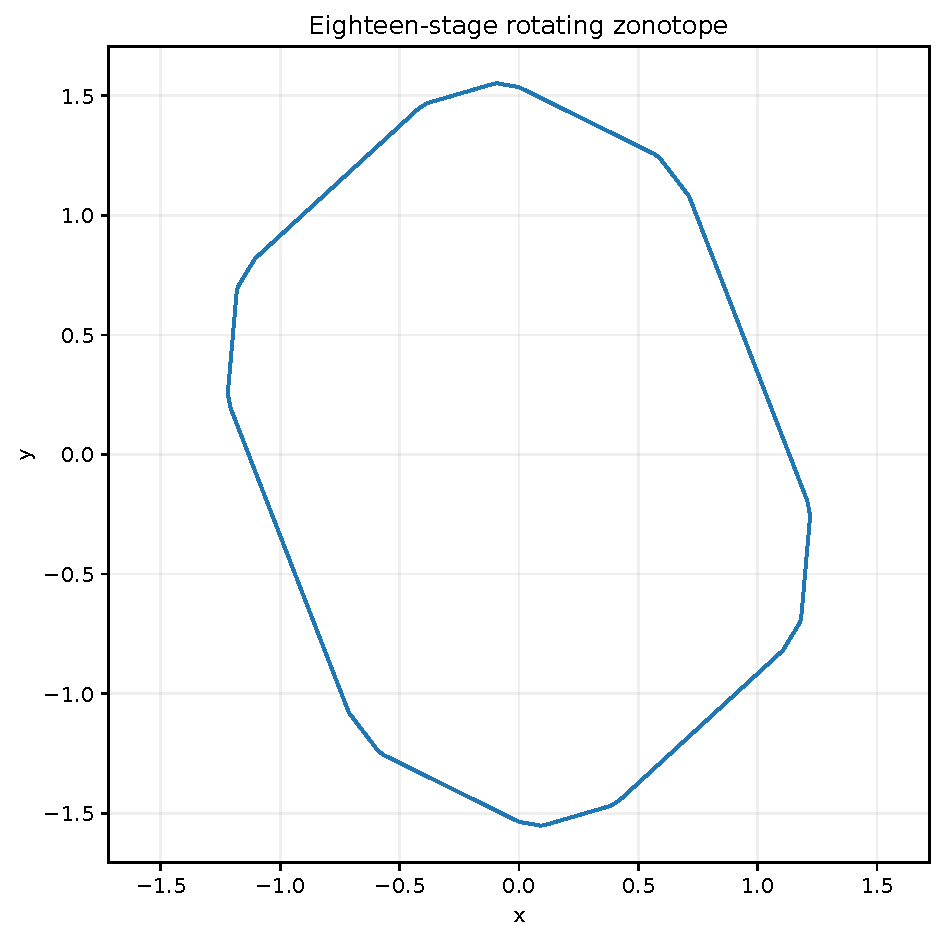
\includegraphics[width=0.74\textwidth]{rotating_zonoid.pdf}
\caption{The $18$-stage support for $q=0.68$ and
$\theta/\pi=(\sqrt5-1)/2$.  The finite polygon already approximates an infinite
zonotope with dense edge directions.}
\label{fig:rotating-zonoid}
\end{figure}

\begin{figure}[H]
\centering
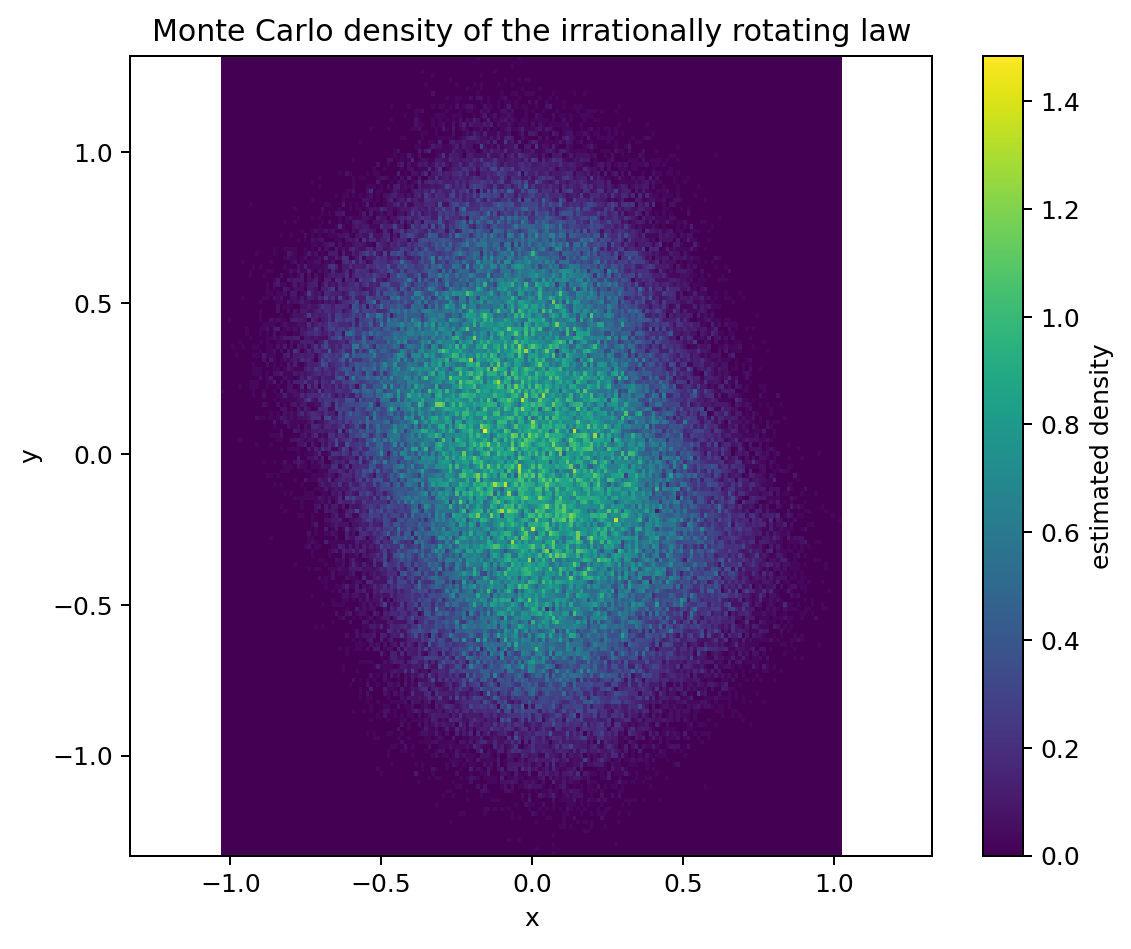
\includegraphics[width=0.78\textwidth]{sample_density.png}
\caption{Monte Carlo density for the same irrationally rotating law.  The
support boundary is infinitely polygonal, while the density is $C^\infty$ by
\cref{thm:smoothness} and log-concave by \cref{thm:logconcavity}.}
\label{fig:sample-density}
\end{figure}

\begin{proposition}[A certified central-plateau regime]
\label{prop:plateau}
\New\ Assume $\sin\theta\ne0$.  Put
\[
 P_2=[-qR_\theta v,qR_\theta v]
     +[-q^2R_{2\theta}v,q^2R_{2\theta}v],
 \qquad
 K_{>2}=\sum_{n\ge3}[-q^nR_{n\theta}v,q^nR_{n\theta}v],
\]
and define the Minkowski erosion
$P_2\ominus K_{>2}=\{x:x-K_{>2}\subseteq P_2\}$.
On this erosion the density is exactly constant:
\begin{equation}
 f(x)=\frac{1}{4a^2q^3|\sin\theta|}.
 \label{eq:plateau-value}
\end{equation}
In particular, if
\begin{equation}
 \frac{q}{1-q}<|\sin\theta|,
 \label{eq:plateau-sufficient}
\end{equation}
then the erosion contains a neighborhood of the origin, so $f$ has a
full-dimensional central plateau and cannot be strictly log-concave.
\end{proposition}

\begin{proof}
The first two digits have the uniform density
$(4|\det(qR_\theta v,q^2R_{2\theta}v)|)^{-1}$ on the parallelogram $P_2$.
Convolution with the tail measure therefore leaves that constant unchanged at
all $x$ for which $x-K_{>2}\subseteq P_2$, proving
\eqref{eq:plateau-value}.  The Euclidean inradius of $P_2$ is
$a q^2|\sin\theta|$, while
$K_{>2}$ lies in the ball of radius $a q^3/(1-q)$.  The strict inequality
\eqref{eq:plateau-sufficient} places the latter ball strictly inside $P_2$ and
makes the erosion have nonempty interior.
\end{proof}

\subsection{Dense edges and an exact curvature measure}

\begin{theorem}[Dense-edge boundary of the irrational support]
\label{thm:dense-edges}
\New\ Suppose $\theta/\pi$ is irrational.  For every $n\ge1$, the boundary of
$K_{q,\theta}$ has exactly two opposite exposed edges parallel to
$R_{n\theta}v$, each of length $2aq^n$.  There are no other nontrivial exposed
faces.  Their directions are dense modulo $\pi$, and the union of their relative
interiors has full arclength measure on $\partial K_{q,\theta}$.
\end{theorem}

\begin{proof}
For a unit normal $u$, the exposed face of a Minkowski sum is the Minkowski sum
of the exposed faces of its summands.  A segment $[-g,g]$ contributes an endpoint
unless $u\perp g$, in which case it contributes the full segment.  Irrationality
ensures that no two generator directions agree modulo $\pi$.  Thus a nontrivial
face occurs exactly when $u$ is perpendicular to one generator, and its length is
$2\Norm{g_n}=2aq^n$.  The directions $n\theta\bmod\pi$ are dense by Weyl's
equidistribution theorem \cite{Weyl}.  The two edges for each $n$ have total
length $4aq^n$; summing gives $4aq/(1-q)$, exactly the perimeter in
\eqref{eq:rotating-perimeter}.  Hence the complement has zero arclength.
\end{proof}

Let $S_K$ be the planar surface-area measure: an edge contributes its length at
its outward unit normal.  The proof gives the atomic measure
\begin{equation}
 S_{K_{q,\theta}}
 =2a\sum_{n\ge1}q^n
 \left(\delta_{n\theta+\varphi_0+\pi/2}
      +\delta_{n\theta+\varphi_0-\pi/2}\right).
 \label{eq:surface-measure}
\end{equation}
With the unnormalized angular Fourier--Stieltjes convention
$\AngularFourierStieltjesCoefficient{S}{k}
=\int\EulerE^{-\ImaginaryUnit k\phi}\Differential S(\phi)$,
\begin{equation}
 \AngularFourierStieltjesCoefficient{S}{k}
 =4a\cos\frac{k\pi}{2}\,
  \EulerE^{-\ImaginaryUnit k\varphi_0}
  \frac{q\EulerE^{-\ImaginaryUnit k\theta}}{1-q\EulerE^{-\ImaginaryUnit k\theta}}.
 \label{eq:surface-fourier}
\end{equation}
Thus the boundary's curvature data are finite cyclotomic resolvents even though
the density inside is governed by an infinite sinc product.

\subsection{Rational functions versus natural boundaries}

The area series introduces
\begin{equation}
 S_\theta(z)=\sum_{m\ge1}\AbsoluteValue{\sin(m\theta)}z^m,
 \qquad |z|<1.
 \label{eq:area-series}
\end{equation}

\begin{theorem}[Rotation-orbit Abel residues]
\label{thm:abel-residues}
\New\ Let $g(x)=\sum_{k\in\IntegerNumbers}c_k\EulerE^{\ImaginaryUnit kx}$ be a continuous periodic
function with $\sum_k|c_k|<\infty$, let $\theta/(2\pi)$ be irrational, and put
\begin{equation}
 G(z)=\sum_{n\ge1}g(n\theta+\delta)z^n.
 \label{eq:orbit-generating}
\end{equation}
Then for every $k\in\IntegerNumbers$,
\begin{equation}
 \lim_{r\uparrow1}(1-r)G(r\EulerE^{-\ImaginaryUnit k\theta})
 =c_k\EulerE^{\ImaginaryUnit k\delta}.
 \label{eq:abel-residue}
\end{equation}
Every point $\EulerE^{-\ImaginaryUnit k\theta}$ for which $c_k\ne0$ is therefore a singularity
of $G$.  If those points are dense on the unit circle, the circle is a natural
boundary.
\end{theorem}

\begin{proof}
Insert the absolutely convergent Fourier series:
\[
 (1-r)G(r\EulerE^{-\ImaginaryUnit k\theta})
 =\sum_{\ell\in\IntegerNumbers}c_\ell\EulerE^{\ImaginaryUnit\ell\delta}
 \frac{(1-r)r\EulerE^{\ImaginaryUnit(\ell-k)\theta}}
      {1-r\EulerE^{\ImaginaryUnit(\ell-k)\theta}}.
\]
The $\ell=k$ term tends to $c_k\EulerE^{\ImaginaryUnit k\delta}$, and every other term tends to
zero because irrationality prevents a unit denominator.  Each fraction has
modulus at most one, so dominated convergence applies using
$\sum|c_\ell|<\infty$.  If $G$ extended holomorphically across the candidate
point, it would be bounded there and the left side would tend to zero, a
contradiction.  Dense singularities exclude continuation across every boundary
arc.
\end{proof}

The absolutely convergent Fourier series
\begin{equation}
 |\sin x|=\frac{2}{\pi}-\frac{4}{\pi}\sum_{k\ge1}
 \frac{\cos(2kx)}{4k^2-1}
 \label{eq:absolute-sine-fourier}
\end{equation}
contains a nonzero coefficient at every even frequency.

\begin{corollary}[Arithmetic dichotomy for rotating area]
\label{cor:natural-boundary}
\New\ If $\theta/\pi\in\RationalNumbers$, the coefficient sequence
$|\sin(m\theta)|$ is periodic, so $S_\theta(z)$ is rational; if
$\theta=\pi a/p$ with integers $a,p$, one may write
\begin{equation}
 S_\theta(z)=
 \frac{\sum_{m=1}^{p}|\sin(m\theta)|z^m}{1-z^p}.
 \label{eq:rational-area-series}
\end{equation}
If $\theta/\pi\notin\RationalNumbers$, the unit circle is a natural boundary of
$S_\theta(z)$ and hence of the analytically continued area in
\eqref{eq:rotating-area}.
\end{corollary}

\begin{proof}
The rational case is periodic summation.  In the irrational case apply
\cref{thm:abel-residues} to \eqref{eq:absolute-sine-fourier}.  The singular
points $\EulerE^{-2\ImaginaryUnit k\theta}$ are dense because $\theta/\pi$ is irrational.
The rational prefactor in \eqref{eq:rotating-area} cannot remove a dense set of
nonzero Abel residues.
\end{proof}

\begin{corollary}[Natural boundary of every directional support series]
\label{cor:support-natural-boundary}
\New\ For irrational $\theta/\pi$ and every fixed direction $\varphi$, the
analytic function
\begin{equation}
 H_{\theta,\varphi}(z)
 =\sum_{n\ge1}\AbsoluteValue{\cos(n\theta+\varphi_0-\varphi)}z^n
 \label{eq:support-series}
\end{equation}
has the unit circle as a natural boundary.
\end{corollary}

\begin{proof}
The Fourier series of $|\cos x|$ is a phase shift of
\eqref{eq:absolute-sine-fourier} and has nonzero coefficients at all even
frequencies.  Apply \cref{thm:abel-residues}.
\end{proof}

\begin{figure}[H]
\centering
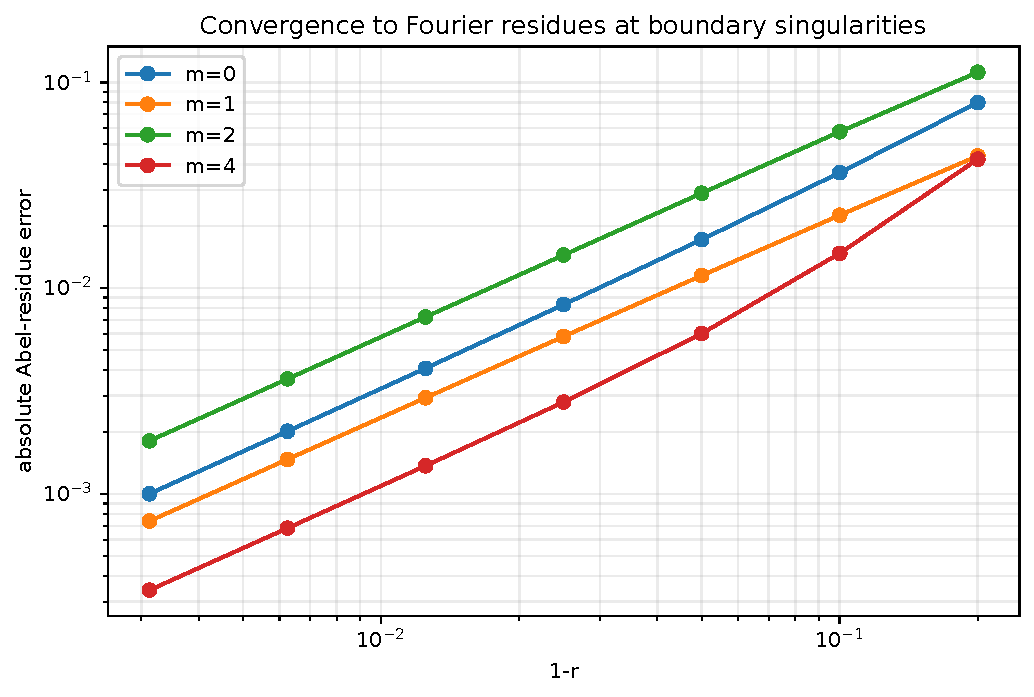
\includegraphics[width=0.78\textwidth]{abel_residue_convergence.pdf}
\caption{Numerical convergence of the Abel residues in
\eqref{eq:abel-residue} for the area series at four dense boundary
singularities.  The limiting constants are the exact Fourier coefficients in
\eqref{eq:absolute-sine-fourier}.}
\label{fig:abel-residues}
\end{figure}

\subsection{An Abel shape theorem: polygons versus a disk}

The natural normalization is
\begin{equation}
 \widetilde K_{q,\theta}:=\frac{1-q}{q}K_{q,\theta};
 \label{eq:shape-rescaling}
\end{equation}
its perimeter is the constant $4a$.

\begin{theorem}[Abel shape limit]
\label{thm:abel-shape}
\New\ As $q\uparrow1$:
\begin{enumerate}
\item if $\theta/\pi$ is irrational, then
\begin{equation}
 \widetilde K_{q,\theta}\longrightarrow
 \{x\in\RealNumbers^2:\Norm x\le 2a/\pi\}
 \label{eq:disk-limit}
\end{equation}
in Hausdorff distance;
\item if $\theta/\pi$ is rational and $p$ is a period modulo $\pi$, then
\begin{equation}
 \widetilde K_{q,\theta}\longrightarrow
 \frac1p\sum_{m=1}^p[-R_{m\theta}v,R_{m\theta}v],
 \label{eq:polygon-limit}
\end{equation}
a finite zonotope.
\end{enumerate}
In the irrational case,
\begin{equation}
 \left(\frac{1-q}{q}\right)^2
 \operatorname{Area}(K_{q,\theta})\longrightarrow\frac{4a^2}{\pi}.
 \label{eq:area-disk-limit}
\end{equation}
\end{theorem}

\begin{proof}
The rescaled support function is
\[
 \widetilde h_q(\varphi)
 =a(1-q)\sum_{n\ge1}q^{n-1}
  |\cos(n\theta+\varphi_0-\varphi)|.
\]
For irrational rotation, insert the absolutely convergent Fourier series of
$|\cos|$.  The constant coefficient contributes $2a/\pi$.  Every nonconstant
mode contains
\[
 \frac{(1-q)\EulerE^{\ImaginaryUnit k\theta}}{1-q\EulerE^{\ImaginaryUnit k\theta}}\longrightarrow0.
\]
Its modulus is at most one, so absolute summability gives convergence uniformly
in $\varphi$.  Uniform convergence of support functions is exactly Hausdorff
convergence of convex bodies.  In the rational case, the Abel means of a periodic
sequence converge to its period average, uniformly in $\varphi$, yielding
\eqref{eq:polygon-limit}.  Area is continuous under Hausdorff convergence, and
the limiting disk has area $\pi(2a/\pi)^2$.
\end{proof}

\begin{figure}[H]
\centering
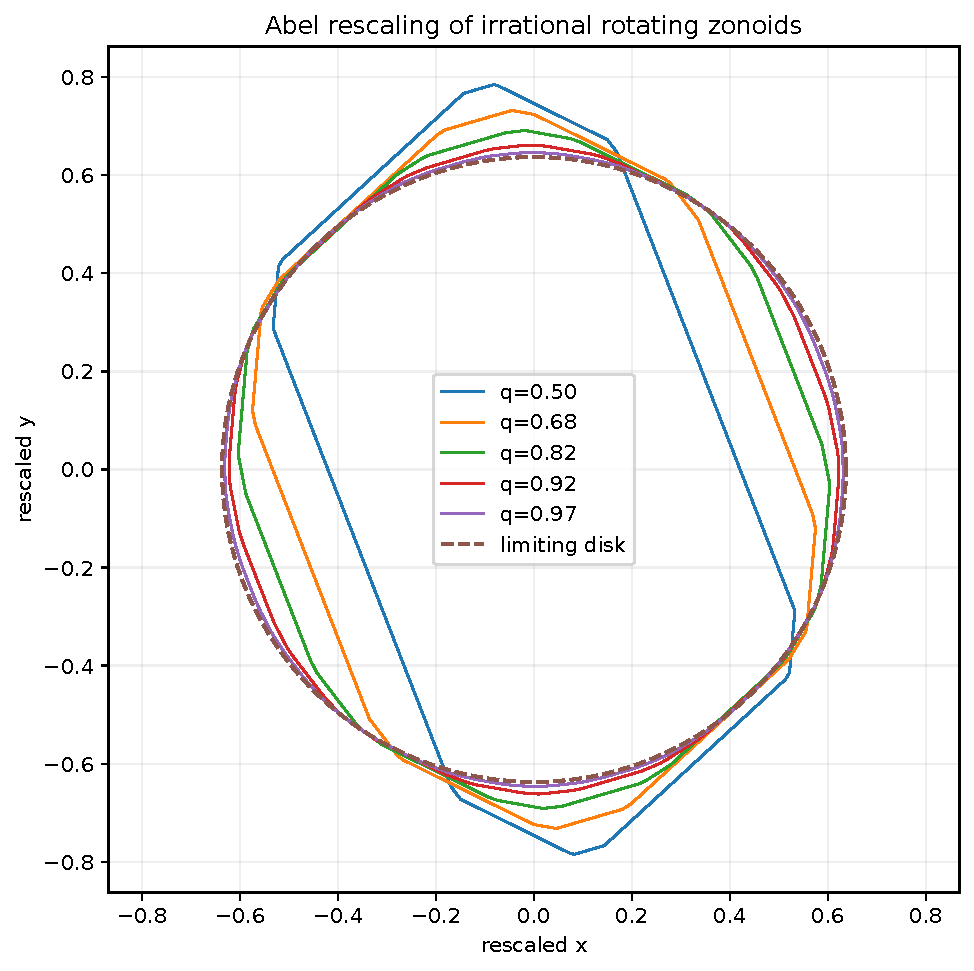
\includegraphics[width=0.78\textwidth]{abel_shape_limit.pdf}
\caption{The rescaled supports $(1-q)K_{q,\theta}/q$ approach the disk of radius
$2/\pi$ for the golden-ratio rotation.  Each finite plot uses enough generators
that its omitted Hausdorff tail is below $2\times10^{-8}$.}
\label{fig:abel-shape}
\end{figure}

\begin{remark}[Geometry remembers arithmetic]
The normalized perimeter is the same in both cases, but the limiting shape
remembers whether the rotation is periodic.  Rational angles retain a finite
directional alphabet and produce a polygon.  Irrational angles equidistribute
the atomic curvature measure \eqref{eq:surface-measure} and produce a disk.
At finite $q$, however, the irrational support still has pure-point curvature
with dense atoms.  Smooth shape appears only after Abel rescaling and passage to
the limit.
\end{remark}

\subsection{Cyclotomic formulas for projection cumulants}

Let $w$ make angle $\varphi$ and put $\delta=\varphi_0-\varphi$.  Then
$\ip{w}{q^nR_{n\theta}v}=a\Norm w q^n\cos(n\theta+\delta)$.  Let
$Q=q^{2m}$.

\begin{proposition}[Finite resolvent formula]
\label{prop:rotating-cumulants}
\New\ For $m\ge1$,
\begin{align}
 \kappa_{2m}(\ip{w}{X_{q,\theta}})
 ={}&c_{2m}(a\Norm w)^{2m}
 \Bigg[
 2^{-2m}\binom{2m}{m}\frac{Q}{1-Q}
 \nonumber\\
 &\quad+2^{1-2m}\sum_{\ell=1}^m\binom{2m}{m-\ell}
 \operatorname{Re}\left(
 \EulerE^{2\ImaginaryUnit\ell\delta}
 \frac{Q\EulerE^{2\ImaginaryUnit\ell\theta}}
      {1-Q\EulerE^{2\ImaginaryUnit\ell\theta}}
 \right)\Bigg].
 \label{eq:rotating-cumulant}
\end{align}
Thus every fixed-order projection cumulant is a finite sum of geometric or
cyclotomic resolvents, even when the full density has no elementary expression.
\end{proposition}

\begin{proof}
Use
\[
 \cos^{2m}x=2^{-2m}\binom{2m}{m}
 +2^{1-2m}\sum_{\ell=1}^m\binom{2m}{m-\ell}\cos(2\ell x)
\]
and sum each geometric Fourier mode over $n\ge1$.
\end{proof}

\begin{example}[Quarter-turn factorization]
If $v=e_1$ and $\theta=\pi/2$, the even and odd digits occupy orthogonal axes:
\begin{align*}
 X_1&=\sum_{k\ge1}(-1)^kq^{2k}U_{2k},\\
 X_2&=\sum_{k\ge1}(-1)^{k-1}q^{2k-1}U_{2k-1}.
\end{align*}
The coordinates are independent scalar geometric-uniform laws with base $q^2$
and different scales.  The support is a rectangle with half-widths
$q^2/(1-q^2)$ and $q/(1-q^2)$, and \eqref{eq:rotating-area} reduces to its area
$4q^3/(1-q^2)^2$.
\end{example}

\begin{figure}[H]
\centering
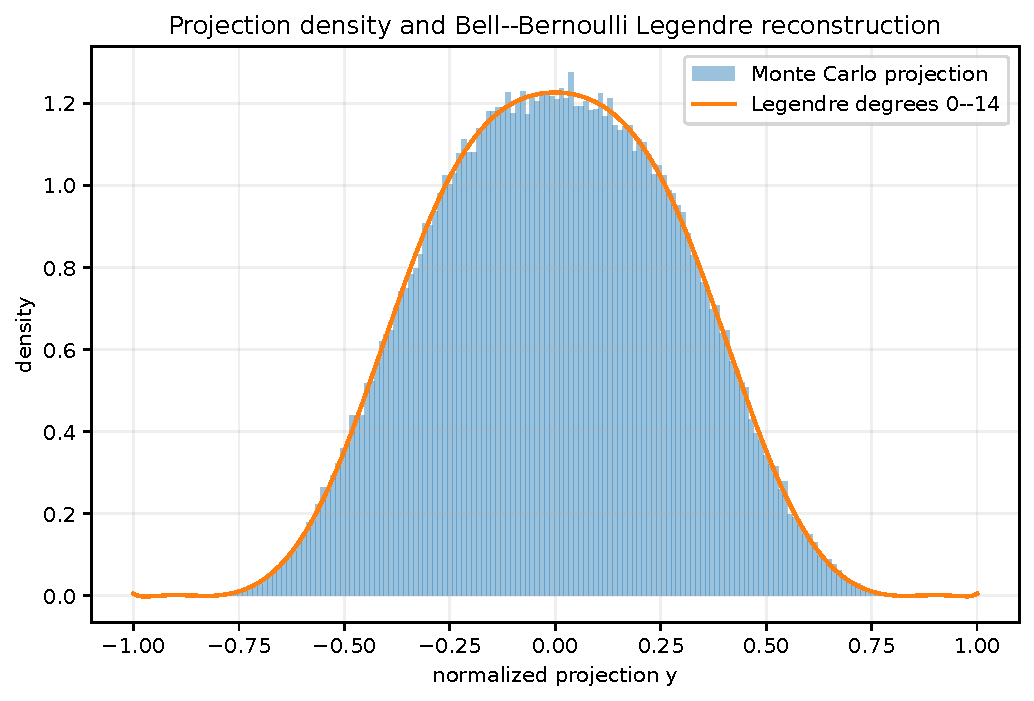
\includegraphics[width=0.78\textwidth]{projection_legendre.pdf}
\caption{A degree-$14$ Legendre reconstruction of one normalized projection,
with coefficients computed from \eqref{eq:rotating-cumulant}, Bell moments, and
\eqref{eq:legendre-coefficient}.  The histogram is independent Monte Carlo data.}
\label{fig:projection-legendre}
\end{figure}

\section{Directional caps, generalized inverse Fabius functions, and Lambert scales}
\markboth{\thesection\quad Directional caps and inverse Fabius scales}{}
\label{sec:caps}

For a direction $w$, let $h=h_K(w)$ and define the deficit from the supporting
hyperplane
\begin{equation}
 D_w=h-\ip{w}{X}\ge0.
 \label{eq:deficit}
\end{equation}
Its distribution function $C_w(x)=\Probability(D_w\le x)$ is a directional analogue of
a Fabius endpoint germ, and $C_w^{-1}$ is a generalized inverse Fabius
quantile.

\begin{theorem}[Exact cap product]
\label{thm:cap-product}
\New\ Put $a_{n,j}=|\ip{w}{B^nv_j}|$.  Then
\begin{equation}
 D_w\overset d=2\sum_{n,j}a_{n,j}V_{n,j},
 \qquad V_{n,j}\stackrel{\mathrm{iid}}\sim\mathrm{Unif}[0,1],
 \label{eq:deficit-series}
\end{equation}
and its Laplace transform is
\begin{equation}
 \mathcal L_w(s):=\Expectation\EulerE^{-sD_w}
 =\prod_{n,j:a_{n,j}>0}
  \frac{1-\EulerE^{-2sa_{n,j}}}{2sa_{n,j}}
 \qquad(s\ge0).
 \label{eq:cap-laplace}
\end{equation}
\end{theorem}

\begin{proof}
For one digit with scalar projection coefficient $b$,
$|b|-bU$ has the same law as $2|b|V$ with $V$ uniform on $[0,1]$.  Independence
then gives the sum and product.
\end{proof}

\begin{corollary}[Rational rotations reduce to finitely many scalar endpoint products]
\label{cor:rational-cap}
\New\ In the rotating planar family, suppose $\theta/\pi$ is rational and let
$p$ be a period of
$c_n=|\cos(n\theta+\delta)|$.  Then
\begin{equation}
 \mathcal L_w(s)
 =\prod_{\substack{1\le r\le p\\ c_r>0}}
  \prod_{k=0}^{\infty}
  \frac{1-\exp(-2sa\Norm w c_rq^{r+kp})}
       {2sa\Norm w c_rq^{r+kp}}.
 \label{eq:rational-cap-factorization}
\end{equation}
Thus a rationally rotating cap is a convolution of finitely many scalar
geometric endpoint laws with common ratio $q^p$.  The scalar saddle and lower
Lambert--$W$ machinery in the repository can be applied factor by factor.
\end{corollary}

\begin{proof}
Group the product \eqref{eq:cap-laplace} by residue class $n\bmod p$.
\end{proof}

For irrational rotations, the amplitudes
$q^n|\cos(n\theta+\delta)|$ have a geometric envelope but a nonperiodic
multiplicative modulation.  The logarithm of the large-argument part of
\eqref{eq:cap-laplace} contains the rotation cocycle
\begin{equation}
 \mathcal C_N(\theta,\delta)
 :=\sum_{n=1}^N\log\bigl(2|\cos(n\theta+\delta)|\bigr).
 \label{eq:rotation-cocycle}
\end{equation}
Its mean is zero, because
$(2\pi)^{-1}\int_0^{2\pi}\log(2|\cos x|)\Differential x=0$, but close returns to the zeros
of cosine can create large negative excursions.  This is the new obstruction to
a literal periodic Lambert correction.

\begin{conjecture}[Diophantine quasiperiodic endpoint law]
\label{conj:diophantine-endpoint}
\Conj\ Suppose $\theta/\pi$ is of bounded continued-fraction type and the phase
$\delta$ is nonresonant.  Put $\lambda=\log(1/q)$.  Then the cap Laplace transform
has
\begin{equation}
 \log\mathcal L_w(s)
 =-\frac{(\log s)^2}{2\lambda}
  +O(\log s\,\log\log s)
 \qquad(s\to\infty),
 \label{eq:conj-log-laplace}
\end{equation}
with a refinement whose nonuniversal term is an explicit smoothing of
$\mathcal C_{\Floor{\log s/\lambda}}(\theta,\delta)$.  After saddle-point
inversion, $C_w(x)$ and $C_w^{-1}(y)$ have the same leading lower-Lambert
skeleton as the scalar geometric law, but the scalar log-periodic carrier is
replaced by a bounded or logarithmically growing quasiperiodic cocycle.
\end{conjecture}

\begin{conjecture}[Liouville resonant spikes]
\label{conj:liouville}
\Conj\ For a dense set of Liouville angles and suitable phases, arbitrarily close
returns to a cosine zero produce subsequences on which the correction to the
quadratic term in \eqref{eq:conj-log-laplace} is larger than any fixed multiple
of $\log\log s$.  Consequently no bounded periodic or quasiperiodic carrier can
give a uniform all-orders endpoint expansion.
\end{conjecture}

\begin{remark}
These conjectures are deliberately weaker than asserting a full expansion.  The
quadratic scale comes from the geometric envelope $q^n$; the unresolved work is
to control the singular Birkhoff sums \eqref{eq:rotation-cocycle} uniformly on
the saddle window.  The problem sits at an intersection of Fabius endpoint
analysis, Sudler-type trigonometric products, Diophantine approximation, and
lower-Lambert inversion.
\end{remark}

\section{Numerical experiments}
\label{sec:numerics}

The archive contains \path{matrix_fabius_experiments.py}, a deterministic,
fully commented program using the seed \texttt{20260830}.  It regenerates all
figures and writes machine-readable CSV tables.  The principal example uses
\[
 q=0.68,
 \qquad
 \frac\theta\pi=\frac{\sqrt5-1}{2},
 \qquad
 v=(1,0).
\]
The irrational angle is of bounded type and gives well-distributed directions.

\subsection{Geometry checks}

The $18$-generator polygon and determinant formulas agree as follows:
\begin{center}
\begin{tabular}{@{}lS[table-format=1.16]@{}}
\toprule
Quantity & {Value} \\
\midrule
polygon area & 5.3337058926631871 \\
determinant-series area & 5.3337058926631880 \\
absolute discrepancy & 0.0000000000000009 \\
polygon perimeter & 8.4917855336588595 \\
generator-sum perimeter & 8.4917855336588612 \\
absolute discrepancy & 0.0000000000000018 \\
infinite area & 5.3447016554636892 \\
infinite perimeter & 8.5000000000000018 \\
\bottomrule
\end{tabular}
\end{center}
The area series was truncated only after a geometric upper bound on the omitted
tail fell below $10^{-16}$.  

\begin{figure}[H]
\centering
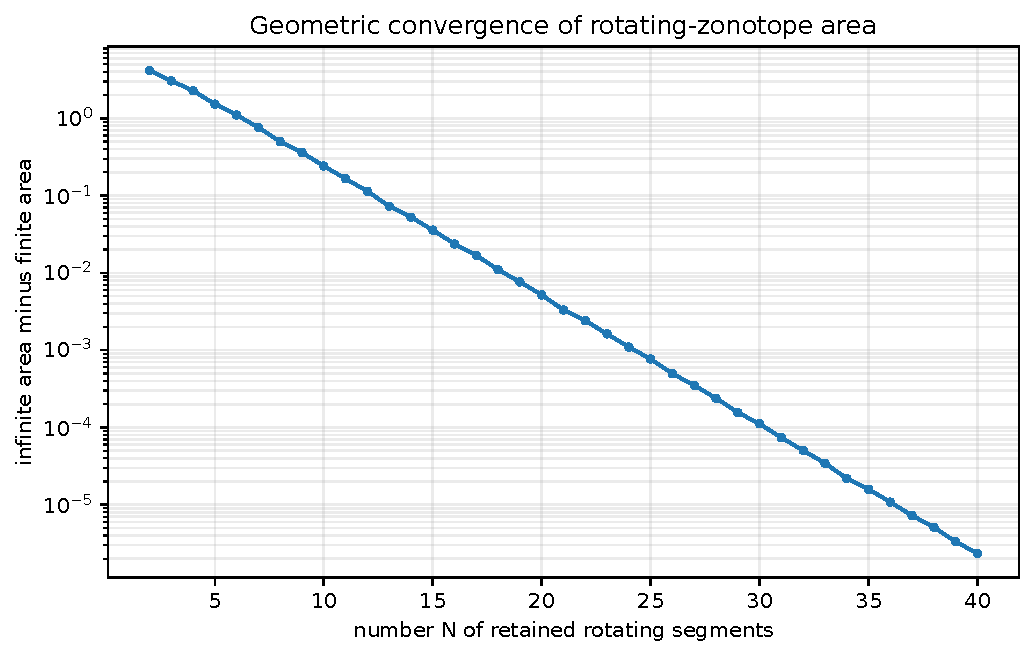
\includegraphics[width=0.78\textwidth]{area_convergence.pdf}
\caption{Convergence of finite support area to the exact infinite series
\eqref{eq:rotating-area}.}
\label{fig:area-convergence}
\end{figure}

\subsection{Fourier, covariance, and Prouhet checks}

For twelve random frequencies, the largest residual in the exact finite-product
identity
\[
 \Phi_N(A^T\xi)=\SincRad\ip{\xi}{v}\Phi_{N-1}(\xi)
\]
was $3.33\times10^{-16}$.  For a six-generator directional Prouhet cube, all
signed moments below degree six vanished with maximum residual
$4.20\times10^{-16}$, and the first surviving degree matched
\eqref{eq:first-tensor} within $2.78\times10^{-16}$.

With 180,000 Monte Carlo samples, the sample covariance was
\[
 \begin{pmatrix}
 0.09506634&-0.02734876\\
 -0.02734876&0.19191718
 \end{pmatrix},
\]
while the exact infinite Lyapunov solution was
\[
 \begin{pmatrix}
 0.09457932&-0.02746051\\
 -0.02746051&0.19212703
 \end{pmatrix}.
\]
The largest entrywise discrepancy, $4.87\times10^{-4}$, is consistent with
ordinary Monte Carlo error.  The direct $28$-generator covariance sum and the
infinite Lyapunov solution agree to the displayed digits.

\subsection{Reproduction command}

From the extracted archive directory, run
\begin{lstlisting}[style=pythonstyle]
python matrix_fabius_experiments.py --output-dir . --samples 180000
\end{lstlisting}
The script creates \path{figures/}, \path{data/}, and \path{results/}.  It uses
no network access and overwrites only its own generated outputs.

\section{Formalization blueprint}
\label{sec:formalization}

The repository already contains reusable probability and infinite-product
infrastructure for absolutely summable vector weights.  The following sequence
would minimize duplication in a Lean formalization.

\subsection{Phase I: generic vector series and support}

Define the matrix weights $g_{n,j}=A^{-n}v_j$ as a flattened summable family.
Reuse the existing arbitrary-vector-weight law to obtain convergence, pushforward
naturality, reflection, and support-as-range.  Add a finite-dimensional lemma
identifying the range with the infinite Minkowski sum and proving
\eqref{eq:support-function}.  The only matrix-specific analytic input is
summability of powers of an expansive inverse.

\subsection{Phase II: sinc products and smoothness}

Instantiate the generalized Rvachev product with linear forms
$z\mapsto\ip{z}{g_{n,j}}$.  Formalize the finite-frame lemma
\cref{lem:block-frame}, then the block-product decay estimate.  The most delicate
step is likely the passage from rapid Fourier decay to a compactly supported
smooth density in several variables; Mathlib's Fourier inversion API may require
a Schwartz-space wrapper.

\subsection{Phase III: distributions and derivative cubes}

Prove \eqref{eq:segment-derivative} first for test functions, then use derivative
and convolution commutation.  The $2^M$ sum should be indexed by
\verb|Fin M -> Bool|; the sign is \verb|(-1) ^ Fintype.card ...| or a direct
parity character.  The tensor Prouhet identity is best formalized from the
factorized exponential polynomial before differentiating at zero.

\subsection{Phase IV: tensor algebra}

Represent order-$k$ tensors as multilinear maps or symmetric powers according to
available library support.  A computationally lighter first tranche can state
all results after contraction with arbitrary $w$; polynomial extensionality then
recovers the tensor identity.  The operator geometric series
\[
 \sum_{n\ge1}(A^{-1})^{\otimes k n}=(A^{\otimes k}-I)^{-1}
\]
is the core reusable lemma.

\subsection{Phase V: planar convex geometry}

The perimeter and area formulas can initially be formalized for finite
zonotopes, followed by monotone limits.  The natural-boundary theorem requires
only an absolutely summable Fourier series and a geometric-series calculation;
it is analytically cleaner than a general natural-boundary criterion.  The Abel
shape theorem reduces to uniform convergence of support functions.

\section{Open problems and further research}
\label{sec:future}

\begin{problem}[Optimal matrix Fourier decay]
\label{prob:optimal-decay}
Determine the sharp directional coefficient in
$-\log|\Phi(tw)|/(\log t)^2$.  For a scalar dilation it is governed by one
logarithmic scale.  For a matrix, the likely invariant is a pressure or joint
Lyapunov quantity built from the orbit of $w$ under $A^{-T}$ and the finite
frame $V$; the block length $L$ in \eqref{eq:log-gaussian} is only a robust upper
bound.
\end{problem}

\begin{problem}[Smith-normal-form moment arithmetic]
For integral $A,V$, determine exact invariant-factor denominator formulas for
joint moments.  The matrices $A^{\otimes 2m}-I$ should play the role occupied by
$2^{2m}-1$ in the dyadic theory.  It is natural to seek matrix $q$-binomial
identities whose denominators are controlled by the Smith normal forms of these
Kronecker powers.
\end{problem}

\begin{problem}[Zero-hyperplane spectral arithmetic]
The zero set of \eqref{eq:fourier-product} is the union of hyperplanes
\[
 \ip{z}{B^nv_j}=k\pi,
 \qquad k\in\IntegerNumbers\setminus\{0\}.
\]
Classify multiplicities and intersections arithmetically.  For rational matrices,
coincidences reduce to lattice relations among rows of powers of $A$; for
rotations, they are controlled by cyclotomic or Diophantine relations.  A
multivariate Jensen formula may turn these arrangements into digit-counting
identities analogous to the scalar zero divisor.
\end{problem}

\begin{problem}[Matrix inverse Fabius geometry]
Develop uniform saddle asymptotics for the directional cap CDF $C_w$ and its
inverse as $w$ crosses normal directions where one or more amplitudes
$|\ip{w}{B^nv_j}|$ vanish.  Rational rotations suggest a finite collection of
Lambert phases; irrational rotations suggest a stratified family of singular
cocycles.
\end{problem}

\begin{problem}[Sharp plateau and strict-log-concavity phase diagram]
\label{prob:plateau-phase}
The non-strict log-concavity is settled by \cref{thm:logconcavity}, while
\cref{prop:plateau} gives a concrete open region of parameters with a flat
core.  Determine the exact set of $(q,\theta)$ for which the rotating density
has a positive-area plateau, and decide whether it is strictly log-concave on
$\operatorname{int}K$ throughout the complementary region.  The rational
phase-locked cases reduce to products and finite convolutions of scalar
geometric-uniform laws; irrational angles require controlling an infinite
sequence of changing box-spline cells.
\end{problem}

\begin{conjecture}[Curvature/density duality]
\label{conj:curvature-density}
\Conj\ In the irrational rotating family, the rate at which the rescaled support
approaches its limiting disk and the rate at which the standardized density
approaches a Gaussian as $q\uparrow1$ are controlled by the same small
denominators $|1-q\EulerE^{2\ImaginaryUnit k\theta}|$.  More precisely, suitable anisotropy norms
of the support function and of the fourth-cumulant tensor should be comparable
up to universal powers of $1-q$ for bounded-type angles.
\end{conjecture}

\begin{problem}[Multivariate polynomial reproduction]
The scalar repository contains exact polynomial synthesis by shifted up-atoms
and Strang--Fix/Appell machinery.  Determine the polynomial reproduction space
of translates of $f_{A,V}$.  The zero-hyperplane arrangement of $\Phi$ should
replace scalar zero multiplicity, while the Appell tensors in
\cref{thm:appell} should give the correction operator.  The answer may depend on
an arithmetic compatibility between $A$, $V$, and the translation lattice.
\end{problem}

\begin{problem}[Noncommuting scale sequences]
Replace the single matrix power $B^n$ by products
$B_1B_2\cdots B_n$ from a finite noncommuting alphabet.  The support remains a
summable infinite zonotope and the derivative cube survives, but the Mahler
equation becomes a cocycle and the cumulant resolvent becomes a transfer-operator
series.  This setting may link the Fabius--Rvachev system to joint spectral
radius, matrix substitution systems, and automatic sequences beyond
Thue--Morse.
\end{problem}

\section{Conclusion}
\label{sec:conclusion}

The scalar Fabius--Rvachev system is not an isolated special function.  It is the
rank-one member of a matrix-dilated family whose probability, harmonic analysis,
convex geometry, arithmetic, and approximation theory remain exactly coupled.
The matrix replacement preserves the decisive mechanisms:
\begin{itemize}
\item uniform digits produce sinc factors and Bernoulli cumulants;
\item dilation produces a Mahler equation and operator resolvents;
\item segment endpoints produce a Thue--Morse cube;
\item finite prefixes are box splines and the limiting density is log-concave;
\item infinite support is a zonoid, with an explicit plateau criterion;
\item projection reduces tensor information to Bell moments and Legendre
      coefficients;
\item directional endpoints recover inverse-Fabius and Lambert-type questions.
\end{itemize}
The rotating planar family shows that this extension is not merely formal.
Arithmetic of the rotation angle is visible simultaneously in the support's
edge directions, its $q$-series area, analytic continuation, Abel shape limit,
projection cumulants, and endpoint cocycle.  Rational rotations give finite
phase decompositions and rational functions; irrational rotations give dense
edges, natural boundaries, and a circular Abel limit.  These phenomena create a
substantial frontier that is adjacent to, but not duplicative of, the repository's
existing scalar and base-$b$ theory.

\appendix

\section{Fourier and tensor conventions}
\label{app:conventions}

The Fourier transform is
\[
 \FourierAngular{f}(-\xi)=\int_{\RealNumbers^d}\EulerE^{\ImaginaryUnit\ip{\xi}{x}}f(x)\Differential x,
 \qquad
 f(x)=\frac1{(2\pi)^d}\int_{\RealNumbers^d}
 \EulerE^{-\ImaginaryUnit\ip{\xi}{x}}\FourierAngular{f}(-\xi)\Differential\xi.
\]
Thus $\FourierAngular{D_gf}(-\xi)=-\ImaginaryUnit\ip{\xi}{g}\FourierAngular{f}(-\xi)$ and
$\FourierAngular{D_g^{2m}f}(-\xi)=(-1)^m\ip{\xi}{g}^{2m}\FourierAngular{f}(-\xi)$.

For vectors $x_1,\ldots,x_k$, normalized symmetrization means
\[
 \Sym(x_1\otimes\cdots\otimes x_k)
 =\frac1{k!}\sum_{\sigma\in S_k}
 x_{\sigma(1)}\otimes\cdots\otimes x_{\sigma(k)}.
\]
Its contraction with $z^{\otimes k}$ is
$\prod_i\ip{z}{x_i}$, which fixes the factor $k!$ in
\eqref{eq:first-tensor}.

\section{A quantitative finite-prefix smoothness lemma}
\label{app:finite-smoothness}

For completeness, here is the finite version implicit in
\cref{thm:Cm-expansion}.  Suppose the first $L$ scales span and choose $p$
consecutive spanning blocks.  From each block, the frame argument selects a
factor satisfying $|\ip{\xi}{g}|\ge c_m\Norm\xi$.  Hence
\[
 |\Phi_{pL}(\xi)|\le C_p(1+\Norm\xi)^{-p}.
\]
If $p>d+k$, then $\Norm\xi^k\Phi_{pL}\in L^1$, so the corresponding finite box
spline is $C^k$.  Additional sinc factors cannot increase the real-axis modulus.
Thus, for any prescribed derivative order, all sufficiently long finite
prefixes possess that order uniformly.  This argument avoids invoking a detailed
combinatorial smoothness theorem for each box-spline direction multiset.

\section{Generated files and numerical ledger}
\label{app:files}

The archive contains:
\begin{center}
\begin{tabularx}{0.95\textwidth}{@{}lX@{}}
\toprule
Path & Purpose \\
\midrule
\path{matrix_dilated_fabius_rvachev.tex} & complete source of this report \\
\path{matrix_dilated_fabius_rvachev.pdf} & compiled report \\
\path{matrix_fabius_experiments.py} & commented deterministic experiment suite \\
\path{requirements.txt} & minimal Python dependency list \\
\path{README.md} & build and reproduction instructions \\
\path{CORPUS_AUDIT.md} & snapshot and novelty ledger \\
\path{figures/*.pdf}, \path{figures/*.png} & vector and raster figures \\
\path{data/area_convergence.csv} & finite/infinite area and perimeter comparison \\
\path{data/abel_residues.csv} & boundary Abel-residue tests \\
\path{data/abel_shape_limit.csv} & support-function distance to the limiting disk \\
\path{data/covariance_check.csv} & Monte Carlo, finite-sum, and Lyapunov covariance \\
\path{data/mahler_checks.csv} & finite matrix-Mahler residuals \\
\path{data/prouhet_checks.csv} & signed moment cancellations \\
\path{data/projection_legendre_coefficients.csv} & exact-formula numerical Legendre coefficients \\
\path{results/numerical_summary.txt} & human-readable audit trail \\
\path{SHA256SUMS} & checksums of archive payloads \\
\bottomrule
\end{tabularx}
\end{center}

\begin{thebibliography}{99}

\bibitem{Anshelevich}
M. Anshelevich,
\newblock Appell polynomials and their relatives,
\newblock \emph{International Mathematics Research Notices} 2004 (2004), no.~65,
3469--3531,
\newblock doi: \url{https://doi.org/10.1155/S107379280413345X}.

\bibitem{Arias}
J. Arias de Reyna,
\newblock An infinitely differentiable function with compact support: definition
and properties,
\newblock English translation of \emph{Rev. Real Acad. Cienc. Exact. Fis. Natur.
Madrid} 76 (1982), 21--38,
\newblock arXiv: \url{https://arxiv.org/abs/1702.05442}.

\bibitem{deBoorBoxSplines}
C. de Boor, K. H\"ollig, and S. Riemenschneider,
\newblock \emph{Box Splines},
\newblock Applied Mathematical Sciences 98, Springer, New York, 1993,
\newblock doi: \url{https://doi.org/10.1007/978-1-4757-2244-4}.

\bibitem{Fabius}
J. Fabius,
\newblock A probabilistic example of a nowhere analytic $C^\infty$-function,
\newblock \emph{Zeitschrift f\"ur Wahrscheinlichkeitstheorie und Verwandte
Gebiete} 5 (1966), 173--174.

\bibitem{GoverKrikorian}
E. Gover and N. Krikorian,
\newblock Determinants and the volumes of parallelotopes and zonotopes,
\newblock \emph{Linear Algebra and its Applications} 433 (2010), 28--40,
\newblock doi: \url{https://doi.org/10.1016/j.laa.2010.01.031}.

\bibitem{JessenWintner}
B. Jessen and A. Wintner,
\newblock Distribution functions and the Riemann zeta function,
\newblock \emph{Transactions of the American Mathematical Society} 38 (1935),
48--88,
\newblock doi: \url{https://doi.org/10.1090/S0002-9947-1935-1501802-5}.

\bibitem{McCullagh}
P. McCullagh,
\newblock Tensor notation and cumulants of polynomials,
\newblock \emph{Biometrika} 71 (1984), 461--476,
\newblock doi: \url{https://doi.org/10.1093/biomet/71.3.461}.

\bibitem{Prekopa}
A. Pr\'ekopa,
\newblock On logarithmic concave measures and functions,
\newblock \emph{Acta Scientiarum Mathematicarum} 34 (1973), 335--343.

\bibitem{ProtasovZaitseva}
V. Yu. Protasov and T. I. Zaitseva,
\newblock Self-affine 2-attractors and tiles,
\newblock \emph{Sbornik: Mathematics} 213 (2022), 794--830,
\newblock doi: \url{https://doi.org/10.1070/SM9682}.

\bibitem{Weyl}
H. Weyl,
\newblock \"Uber die Gleichverteilung von Zahlen mod Eins,
\newblock \emph{Mathematische Annalen} 77 (1916), 313--352,
\newblock doi: \url{https://doi.org/10.1007/BF01475864}.

\bibitem{Repository}
V. Reshetnikov,
\newblock \texttt{ProveIt}: Fabius function formalization and research documents,
\newblock snapshot \texttt{90b2d3587833dea1bc4a6bf0c36d92f7200396e6},
\newblock \url{https://github.com/VladimirReshetnikov/ProveIt/tree/main/Analysis/FabiusFunction}.

\end{thebibliography}

\end{document}
